\documentclass{llncs}
\usepackage{graphicx}
\usepackage[T1]{fontenc}
\usepackage{lmodern}
\usepackage{url}
\usepackage{textcomp}
\usepackage{amsmath}
\usepackage{amssymb}
\usepackage{hyperref}
\usepackage[authoryear,round]{natbib}
\usepackage{longtable,booktabs,array}
\usepackage{calc} % for calculating minipage widths
% Correct order of tables after \paragraph or \subparagraph
\usepackage{etoolbox}
\makeatletter
\patchcmd\longtable{\par}{\if@noskipsec\mbox{}\fi\par}{}{}
\makeatother

\usepackage{color}
\usepackage{fancyvrb}
\DefineVerbatimEnvironment{Highlighting}{Verbatim}{commandchars=\\\{\}}
\newenvironment{Shaded}{}{}
\newcommand{\Program}{\mathcal P}
\newcommand{\ru}{r}
\newcommand{\naf}{not}
\newcommand{\answerSet}{\mathcal M^\Program}
\newcommand{\answerSetReduct}{\mathcal M^{\reductP}}
\newcommand{\groundLitP}{Lit}
\newcommand{\subsetReduct}{\mathcal R}
\newcommand{\reductP}{\mathcal P^{\mathcal R}}
\newcommand{\modelX}{\mathcal X}
\newcommand{\modelY}{\mathcal Y}
\newcommand{\NormalTok}[1]{#1}
\providecommand{\tightlist}{%
  \setlength{\itemsep}{0pt}\setlength{\parskip}{0pt}}

%%
\title{Prompt Framing Sensitivity in Large Language Models for Code and Reasoning Tasks}
\author{Duc Toan Huynh}
\institute{ M.Sc. Data Science, University of Europe for Applied Sciences\\
Supervisors: Prof.~Dr.~Iftikhar Ahmed and Dr.~Sami ur Rahman}

\begin{document}
\maketitle

\begin{abstract}
LLMs are increasingly used in coding assistants and agentic workflows, where small prompt-framing choices affect parser compatibility, verbosity, latency, and correctness. However, common advice about tone, role assignment, and formats like JSON or XML remains under-tested across models and tasks.

This paper examines prompt-framing effects through a full-factorial experiment with 18 prompt variants (3 tones x 2 roles x 3 formats). With 50 base tasks per task kind (Python code generation and mathematical reasoning), we conducted 1,800 runs per model across 6 local and 2 cloud LLMs, 14,400 runs in total. We measure Pass@1 correctness, duration, completion tokens, and output compliance.

Results show that model ability dominates correctness, while prompt effects are smaller, task-specific, and model-specific. Nemotron and DeepSeek strongly skew pooled averages. A mixed-effects logistic analysis with base-task random intercepts confirms the main contrasts. Prompt framing affects behaviors more than correctness: polite prompts increase output length, expert role framing slightly hurts cloud model performance, and JSON reduces the math pass rate for local models. In contrast, structured formats (JSON/XML) improve pass rates in API Python code generation.

The study found no universal prompting technique that reliably improves model performance. A strategy that helps one model may hurt another. Therefore, prompt engineers should test policies on their target models, instead of using universal prompt advice. Reliable LLM-based coding systems need explicit output constraints, robust parsers, validation loops, and local prompt-policy testing.

\end{abstract}

\begin{keywords}
Large Language Models, Prompt Engineering, Code Generation, Mathematical Reasoning, Empirical Software Engineering

\end{keywords}


\section{Introduction}\label{sec:introduction}

    Large Language Models (LLMs) are widely used as assistants for software engineering work: planning, code generation, debugging, test generation/ automation, documentation, and agentic tool workflows \citep{brown2020fewshot, ouyang2022instructgpt, chen2021codex, jimenez2023swebench}. In those systems, models' responses are passed to a parser, executed by a test harness, extracted into a function body, checked by an automated judge, or used as input to another tool. Therefore, not only the correctness but also the surface behavior matters. A response may contain the right algorithm but still fail because the harness cannot parse: it may include extra markdown, explanations, invalid JSON/XML, no clear final answer, or text that the evaluation pipeline cannot easily extract.

    Those settings make prompt framing an important part of system design. Developers often use techniques such as polite language, assigning expert roles, pressuring for accuracy, or formatting the prompt in JSON or XML \citep{li2023emotionprompt,yin2024politeness,liu2024structuredoutput}. Such common advice may be useful in some context, but evidence of the effectiveness of many prompt rules is not strong. Prior work shows that prompt wording, formatting, and ordering can change model behavior in different directions \citep{zhao2021calibrate, lu2021fantastically, sclar2023spurious, zhuo2024prosa}. A prompt that improves one model on one task may fail on another model or task. A prompt that helps a cloud model return parseable code may harm a local math model by encouraging compact answers. A role prompt may clarify the domain expectation for one model, but may make another model more verbose.

    This led to two problems. The first problem is the reproducibility problem for empirical LLM research. If prompt phrasing changes model behavior in ways that are not reported or controlled, the results' performance may be caused by prompt design rather than model ability \citep{hua2025promptartifact}. The second problem is the reliability problem for coding agents. If prompt choices are selected from folklore rather than experiment and validation, an engineering workflow may become slower, more expensive, less parsable, or produce more errors.

    This paper studies prompt framing sensitivity: how semantically similar prompts lead to different behaviors due to framing choices. We examine three factors: tone (neutral, polite, aggressive), role (no role and expert role), and input format (plaintext, JSON, XML). These three factors create an 18-category prompt matrix, and each base task is evaluated under every category, across coding and mathematical reasoning tasks.\\

    The main software-engineering task is Python code generation. The task asks the model to generate Python code satisfying given requirements; an evaluator then extracts the code from the response and evaluates it against a list of tests. The secondary domain is mathematical reasoning, where only the final answer will be extracted and evaluated. The distinction matters: code workflows often benefit from clean, parseable output, whereas in math only the final number matters, even though deriving it may require enough space for intermediate reasoning.

    The main finding of this study is deliberately conservative. Model ability dominates task performance, but prompting still has effects: it changes verbosity, latency, result-only compliance, and sometimes Pass@1 rate. However, the effects depend on task type, model, and evaluators. A neutral tone or polite words do not always help; the same holds for expert roles and structured formats. Therefore, prompt policies should be tested in specific setups: model, tasks, parser, evaluator, latency requirement, and other constraints of the target system.

    This paper is guided by four questions regarding the size of prompt-framing effects, their impact on specific tasks and models, changes in observable behavior, and how relevant behavioral factors contribute to explaining differences in correctness. The research questions are outlined in Section~\ref{research-questions}.

    This paper makes four contributions:

\begin{itemize}
\tightlist
\item
  A systematic experiment: full-factorial prompt-framing experiment combining tone, role framing, and prompt format across 14,400 LLM runs.
\item
  Evaluating beyond correctness alone: A joint evaluation of both correctness and observable behaviors, following the broader view that LLM evaluation should track multiple outcomes such as response length, speed, and compliance, rather than accuracy alone \citep{liang2023helm}.
\item
  Model- and task-stratified analysis: Rather than only reporting aggregate results, we also report results separately for each model and task category, showing that prompt effects are smaller than model effects but still meaningful for output behavior and engineering reliability.
\item
  Mediation and sensitivity analysis: we examine when prompt effects are associated with verbosity, compliance, and runtime, and when pooled averages are dominated by a single strong model.
\end{itemize}


\section{Related Work}\label{sec:relatedwork}

\subsection{Prompt Sensitivity and Prompt Engineering in
LLMs}\label{prompt-sensitivity-and-prompt-engineering-in-llms}

Since large language models with strong few-shot and instruction-following abilities appeared in 2020, prompt engineering has become an essential part of working with these models \citep{brown2020fewshot}. Recently, prompting techniques have evolved from simple task descriptions to include instructions, examples, input/output format, role descriptions, reasoning cues, and conversational style. Recent surveys describe prompt engineering not as a collection of standard rules but as a broad and heterogeneous design space with many proposed techniques \citep{schulhoff2024promptreport}.

Early research on prompt-programming and few-shot calibration work also showed that prompts are not merely presentation layers but can significantly influence model behaviors. Reynolds and McDonell describe prompts as natural-language programs that communicate task intention and structure \citep{reynolds2021promptprogramming}. Zhao et al. demonstrated that prompt format, example choice, and example order can create a large variance in few-shot accuracy \citep{zhao2021calibrate}. Lu et al. found that prompt example permutations alone can change performance from near-random to near state-of-the-art \citep{lu2021fantastically}. More recent work extended these findings to superficial prompt features. Sclar et al. showed that minor formatting changes such as spacing and delimiter choice can cause significant performance shifts \citep{sclar2023spurious}. Zhu et al. evaluated model robustness under adversarial prompt perturbations \citep{zhu2023promptrobust}, and Zhuo et al. studied how prompt structure affects code-generation evaluation \citep{zhuo2024prosa}. Together, these results motivate treating prompts as part of the experimental setup rather than as incidental text.

However, much of the prompt-sensitivity work focuses primarily on final accuracy. In a production software application, accuracy is an essential but not sufficient condition. A response might provide correct output but be overly wordy for rapid processing, delayed, or organized in a manner that makes extraction difficult. Therefore, the paper distinguishes correctness from output behavior, which can be measured using variables such as token count, duration, result-only compliance, blank responses, and extraction failures.

Tone and social framing are also relevant. Studies on emotional stimuli have shown that emotion-oriented discourse can improve the quality of generated messages \citep{li2023emotionprompt}, while the findings of politeness studies indicate that polite language can influence the content and style of responses \citep{yin2024politeness}. These findings justify including tone as a prompt factor, but they do not support general rules. In other words, a polite prompt facilitating accuracy in one setting may lead to verbosity or response latency in another context.

\subsection{LLMs for Code Generation and Software-Engineering
Tasks}\label{llms-for-code-generation-and-software-engineering-tasks}

Code generation is the main software engineering application of LLMs. Benchmarks such as HumanEval and MBPP evaluate whether generated Python programs satisfy hidden or visible tests \citep{chen2021codex, austin2021mbpp}. For  more realistic scenarios, SWE-bench extends evaluation to the repository level \citep{jimenez2023swebench}. Those evaluations measure function correctness objectively rather than subjective preference. They also reveal a practical problem in evaluation: they depend on the process of extraction and executing the code from model responses. Therefore, generated code must be well recognizable, syntactically correct, and compatible with the test suites.

For these reasons, code generation is particularly suitable for studying prompt framing. In programming workflows, useful products are often not explanations, but functions, patches, commands, or structured outputs. Prompt framing affects whether the model returns clean code, code wrapped with markdown, text with code, or malformed output. A prompt can therefore change the pass rate by changing parser compatibility, even when the model's ability to solve the task is unchanged.

This study uses small, controlled Python tasks rather than repository-level tasks: task difficulty stays constant while framing changes, so prompt effects can be isolated. Section~\ref{tasks} discusses what this design does and does not represent.

\subsection{Structured Prompts, Output Constraints, and Parser
Compatibility}\label{structured-prompts-output-constraints-and-parser-compatibility}

Structured prompts and output constraints are common techniques in LLM applications. Developers often use JSON, XML, schemas, field labels, or strict response instructions to make outputs easier to parse \citep{liu2024structuredoutput}. Structured output can improve compatibility with software systems, but it does not automatically yield positive results. Just wrapping input in XML/JSON does not ensure that the model will produce valid structured output, and heavy formatting sometimes makes the model drop useful context or truncate its reasoning.

This study tests plaintext, JSON, or XML input format as a prompt framing factor. Rather than asking only whether a structured format improves accuracy, we investigate the full impact of formatting: whether format shifts both behavior and correctness, and whether those shifts depend on the model and the task (Python code versus math). The results reveal a clear distinction: structuring helps Python API tasks perform better, but JSON reduces local math performance.

This differentiation matters as users frequently mistake input wrapping for output control. Users may submit their tasks in JSON format while requesting that the model produce code or final numbers. In such cases, wrapping serves as a type of input framework as opposed to ensuring a certain output form. The research tackles this issue by tracking both the correctness (pass rate) and structural compliance (e.g., result-only or code-only) of the replies.

In the context of software engineering, this distinction changes how engineers design their pipelines, not just the terminology they use. While wrapping prompts in JSON/XML makes it easier to read/write and inspect, it doesn't guarantee the format of the model response. The model may still generate text, markdown, code, or broken structures. Therefore, downstream tools need both prompt site formatting constraints and output side validation checks. This study treats wrapper formats as a part of this broader model-tool interface.

\subsection{Evaluation of Reasoning and Final-Answer
Extraction}\label{evaluation-of-reasoning-and-final-answer-extraction}

Benchmarks of mathematical reasoning like GSM8K assess whether models are capable of providing correct solutions to word problems \citep{cobbe2021gsm8k}. Research on reasoning prompts, like zero-shot reasoning and chain-of-thought, has shown that prompts have an effect on multi-step reasoning \citep{wei2022cot, kojima2022zeroshot}, though final-answer evaluation still requires extraction, normalization, and comparison. Additionally, reasoning traces may not accurately reflect what the model actually computed \citep{turpin2023unfaithful}. This creates a possible validity issue: an evaluator may be overly strict, too lenient, or sensitive to formatting instead of reasoning quality.

In this study, math problems serve as a secondary validation domain with a different output contract: code tasks reward executable artifacts and parser compatibility, whereas math tasks require deriving a correct answer even when the final output must be compact.

The mathematics perspective aids in distinguishing between two easily confused concepts. Instructions that require only the answer to be submitted may lead to easier evaluation; however, this does not imply that the derivation of the solution is any simpler. On the other hand, reasoning that is visible in the output does not imply that the internal thought process behind the solution is faithful. Therefore, in this paper, longer answers are not automatically treated as better, and shorter answers are not automatically treated as worse. The main findings report the observed relationship among prompt format, answer length, level of compliance, and correctness of the final answer.

\subsection{Research Gap}\label{research-gap}

Table~\ref{tab:related-work-comparison} positions the current study within previous research across relevant dimensions. Three key insights emerge. First, the literature on prompt sensitivity primarily focuses on isolated parameters: Sclar et al. \citep{sclar2023spurious} examine various surface formatting, Lu et al. \citep{lu2021fantastically} experiment with example order, and tone-related studies \citep{li2023emotionprompt,yin2024politeness} differentiate between emotional and politeness framing. However, none of these combine tone, role, and wrapper format within a single factorial design, meaning interactions between these factors remain undetected. Second, while prior research on prompt sensitivity includes code generation studies \citep{zhuo2024prosa}, it fails to integrate these with reasoning domains, behavioral outcomes beyond accuracy, or mediation-style analyses to explain observed differences. Third, broad multi-metric evaluations like HELM \citep{liang2023helm} measure behaviors beyond accuracy but do not isolate prompt framing as the experimental variable. Furthermore, the most relevant tone studies report only accuracy, leaving the cost, latency, and compliance aspects of prompt framing unquantified.

{\footnotesize
\begin{longtable}[]{@{}lccccccccc@{}}
\caption{Comparison with the closest prior studies. \checkmark{} = included, $\sim$ = partial or single-family, -- = not included. Behavioral = outcomes beyond accuracy (tokens, latency, compliance).}\label{tab:related-work-comparison}\tabularnewline
\toprule\noalign{}
Study & Multi & Tone & Role & Format & Code & Reas. & Behav. & Factorial & Repro. \\
\midrule\noalign{}
\endfirsthead
\toprule\noalign{}
Study & Multi & Tone & Role & Format & Code & Reas. & Behav. & Factorial & Repro. \\
\midrule\noalign{}
\endhead
\bottomrule\noalign{}
\endlastfoot
Zhao et al.~\citep{zhao2021calibrate} & $\sim$ & -- & -- & \checkmark & -- & -- & -- & -- & -- \\
Lu et al.~\citep{lu2021fantastically} & $\sim$ & -- & -- & $\sim$ & -- & -- & -- & -- & $\sim$ \\
Sclar et al.~\citep{sclar2023spurious} & \checkmark & -- & -- & \checkmark & -- & -- & -- & $\sim$ & \checkmark \\
Zhu et al.~\citep{zhu2023promptrobust} & \checkmark & -- & -- & $\sim$ & -- & -- & -- & -- & \checkmark \\
Li et al.~\citep{li2023emotionprompt} & \checkmark & $\sim$ & -- & -- & -- & $\sim$ & -- & -- & $\sim$ \\
Yin et al.~\citep{yin2024politeness} & \checkmark & \checkmark & -- & -- & -- & $\sim$ & -- & $\sim$ & $\sim$ \\
Zhuo et al.~\citep{zhuo2024prosa} & \checkmark & -- & -- & \checkmark & \checkmark & -- & -- & $\sim$ & $\sim$ \\
Liang et al.~\citep{liang2023helm} & \checkmark & -- & -- & -- & \checkmark & \checkmark & \checkmark & -- & \checkmark \\
\textbf{This study} & \checkmark & \checkmark & \checkmark & \checkmark & \checkmark & \checkmark & \checkmark & \checkmark & \checkmark \\
\end{longtable}
}

Beyond these studies, this paper also contributes: (i) a comprehensive factorial assessment of tone, role framing, and format (18 variations), thus measuring each factor against a stable baseline instead of in isolation; (ii) an analysis of 8 models ranging from local Ollama deployment systems to hosted APIs, treated as complementary settings rather than pooled benchmarks; (iii) an evaluation of executable code as well as math verification for the final answer under the same prompt matrix; (iv) behavioral outcomes (tokens, time, result-only compliance, and failure modes) reported together with pass@1 and a mediation-style decomposition in associational terms; and (v) mixed-effects inferential analysis, dominant-model sensitivity checks, and public replication materials. The authors consider the approach useful in terms of understanding how prompt framing functions, but not as a general mechanism for ensuring reliability.

\section{Experimental Design}\label{experimental-design}

\subsection{Research Questions}\label{research-questions}

    In this study, we investigate four  research questions:

\begin{itemize}
\tightlist
\item
  RQ1: How large are prompt-framing effects relative to model effects for code-generation and math-reasoning tasks?
\item
  RQ2: Do tone, role framing, and prompt-wrapper format affect correctness, and are effects consistent across task kinds and model families?
\item
  RQ3: How do prompt factors affect observable behavior such as completion tokens, duration, result-only compliance, empty responses, and extraction failures?
\item
  RQ4: To what extent are correctness effects explained by behavioral variables such as verbosity, result-only compliance, and duration?
\end{itemize}

\subsection{Factorial Prompt Design}\label{factorial-prompt-design}

This study adopts a 3 x 2 x 3 factorial design with three tones (neutral, polite, aggressive), two role-framing levels (no role, expert/developer role), and three prompt formats (plain text, JSON, XML), creating 18 prompt variants for each base task.

\begin{longtable}[]{@{}
  >{\raggedright\arraybackslash}p{(\linewidth - 4\tabcolsep) * \real{0.3333}}
  >{\raggedright\arraybackslash}p{(\linewidth - 4\tabcolsep) * \real{0.3333}}
  >{\raggedright\arraybackslash}p{(\linewidth - 4\tabcolsep) * \real{0.3333}}@{}}
\caption{Prompt framing factors and levels.}\tabularnewline
\toprule\noalign{}
\begin{minipage}[b]{\linewidth}\raggedright
Factor
\end{minipage} & \begin{minipage}[b]{\linewidth}\raggedright
Levels
\end{minipage} & \begin{minipage}[b]{\linewidth}\raggedright
Purpose
\end{minipage} \\
\midrule\noalign{}
\endfirsthead
\toprule\noalign{}
\begin{minipage}[b]{\linewidth}\raggedright
Factor
\end{minipage} & \begin{minipage}[b]{\linewidth}\raggedright
Levels
\end{minipage} & \begin{minipage}[b]{\linewidth}\raggedright
Purpose
\end{minipage} \\
\midrule\noalign{}
\endhead
\bottomrule\noalign{}
\endlastfoot
Tone & Neutral, Polite, Aggressive & Test social framing and pressure cues \\
Role Framing & No Role, Expert/Developer Role & Test role/domain framing \\
Wrapper Format & Plain Text, JSON, XML & Test structured prompt wrapping \\
\end{longtable}

Task content remains the same across variants, only framing changes. The \texttt{Format} column in the prompt matrix determines how the task is formatted (plaintext, JSON, XML). It is therefore a prompt format, not a guaranteed structured output. Full prompt templates are treated as replication documentation, rather than fully posted in the main content.

Below is a compact prompt skeleton to illustrate the intervention. Within each task kind, the same base problem text is inserted into the \texttt{task} slot for each of 18 variants. The variable cells change the instruction phrasing via tone and role framing, and also change whether the same instruction/task pair is represented as plaintext, JSON, or XML. Output-only constraints for the API runs are applied separately via system prompts, not as fields in the prompt matrix.

\begin{Shaded}
\begin{Highlighting}[]
\NormalTok{Plaintext:}
\NormalTok{\{role/background sentence\}}
\NormalTok{\{neutral, polite, or aggressive task instruction\}}
\NormalTok{Task: \{PYTHON\_PROBLEM or MATH\_PROBLEM\}}
\NormalTok{}
\NormalTok{JSON:}
\NormalTok{\{}
\NormalTok{  "instruction": "\{role/background sentence + task instruction\}",}
\NormalTok{  "task": "\{PYTHON\_PROBLEM or MATH\_PROBLEM\}"}
\NormalTok{\}}
\NormalTok{}
\NormalTok{XML:}
\NormalTok{\textless{}prompt\textgreater{}}
\NormalTok{  \textless{}instruction\textgreater{}\{role/background sentence + task instruction\}\textless{}/instruction\textgreater{}}
\NormalTok{  \textless{}task\textgreater{}\{PYTHON\_PROBLEM or MATH\_PROBLEM\}\textless{}/task\textgreater{}}
\NormalTok{\textless{}/prompt\textgreater{}}
\end{Highlighting}
\end{Shaded}

The experimental factors were intentionally designed to reflect normal user behavior rather than adversarial attacks. The polite prompts use grateful wording, the aggressive prompts apply pressure, the role prompts assign realistic personas, and the structured prompts wrap the task in JSON or XML. Consequently, the current research uses standard prompt engineering methods rather than red-team perturbation methods. Since every baseline task occurs in all variants, each attribute comparison evaluates output for the same underlying task distribution.

The crossed design also helps address an issue inherent to prompt comparison experiments: concurrently altering multiple factors. In manual prompt tuning, developers frequently change tone, amount of detail, prompt length, and format simultaneously. While such a prompt may lead to practical results, it is difficult to determine which component of the prompt was responsible for the effect. By separating tone, roles, and the wrapper format, our approach enables measuring each of the elements against a stable baseline while preserving realistic prompts.

Figure ~\ref{fig:experimental_pipeline} summarizes the end-to-end experimental pipeline from task sources through prompt construction, model execution, extraction, evaluation, and analysis.

\begin{figure}
\centering
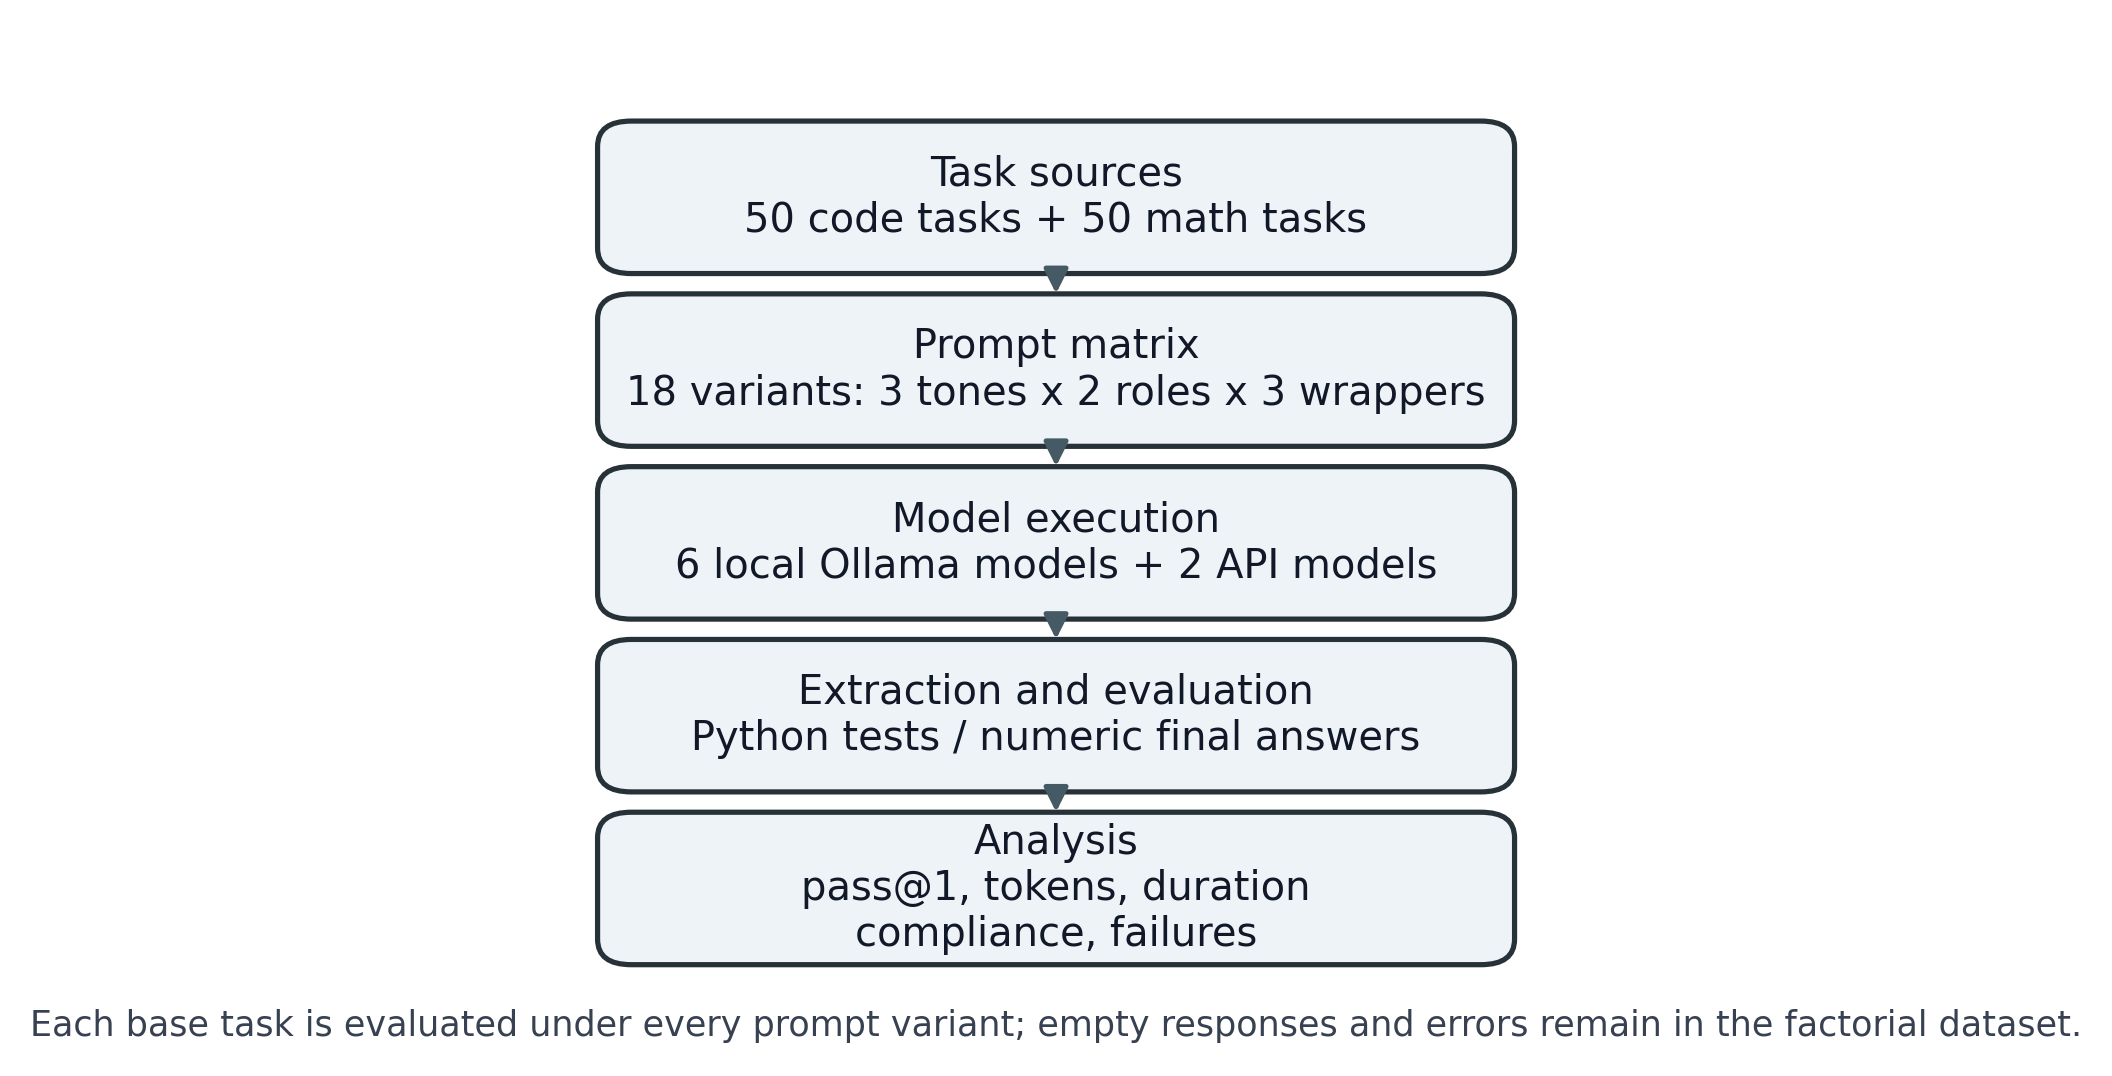
\includegraphics[width=0.95\linewidth,height=\textheight,keepaspectratio,alt={Experimental pipeline from task sources through the prompt matrix, model execution, extraction/evaluation, and analysis.}]{figures/experimental_pipeline.png}
\caption{Experimental pipeline from task sources through the prompt
matrix, model execution, extraction/evaluation, and analysis.}
\label{fig:experimental_pipeline}
\end{figure}

\subsection{Models}\label{models}

The experiment includes two model groups: local models and cloud models (or API models). The local group contains six Ollama-hosted models:

\begin{longtable}[]{@{}lrr@{}}
\caption{Local Ollama models evaluated in the
experiment.}\tabularnewline
\toprule\noalign{}
Model & Parameters & Ollama package size \\
\midrule\noalign{}
\endfirsthead
\toprule\noalign{}
Model & Parameters & Ollama package size \\
\midrule\noalign{}
\endhead
\bottomrule\noalign{}
\endlastfoot
nemotron-3-nano:4b & 3.97B & 2.64 GiB \\
deepseek-coder:6.7b & 6.74B & 3.57 GiB \\
qwen2.5:7b & 7.0B & 4.36 GiB \\
mistral:7b-instruct & 7.24B & 4.07 GiB \\
llama3.1:8b & 8.0B & 4.58 GiB \\
gemma2:9b & 9.0B & 5.07 GiB \\
\end{longtable}

The local package sizes are quantized Ollama package sizes, not FP16 memory requirements. Model identifiers and public model-card information are used for the local model descriptions where available \citep{nemotron3nano2026, deepseekcoder2023, qwen25release2024, mistral7b2023, llama31modelcard2024, gemma2release2024}.

The API group contains two cloud models:

\begin{longtable}[]{@{}ll@{}}
\caption{Cloud API models evaluated in the experiment.}\tabularnewline
\toprule\noalign{}
Reporting label & API model identifier \\
\midrule\noalign{}
\endfirsthead
\toprule\noalign{}
Reporting label & API model identifier \\
\midrule\noalign{}
\endhead
\bottomrule\noalign{}
\endlastfoot
Gemini Flash & \texttt{gemini-3.1-flash-lite-preview} \\
DeepSeek V4 Flash & \texttt{deepseek-ai/DeepSeek-V4-Flash} \\
\end{longtable}

Local and API models are reported separately because they differ in deployment settings, latency, response style, training and post-training procedures, serving infrastructure, and overall capability. Because these differences are confounded with the deployment regime itself, performance gaps between the two groups cannot be attributed to model ability alone.

The models were selected intentionally heterogeneous. The six local models represent lightweight, open source deployments that a practitioner could run through Ollama, while the two API models represent commercial systems with stronger infrastructure and different serving behavior. This split is not to rank all available LLMs or create a general benchmark. It is used to test whether the effects of prompt-factor patterns remain stable when moving between different local and cloud settings. As the results show, stability cannot be assumed.

Separating local and API results also protects the validity of latency and output behavior. Local runtimes are governed by local inference stacks and quantized weights, whereas API runtimes are influenced by hosted serving infrastructure and network conditions. Combining them into a single timing metric would be misleading. Therefore this paper treats local and API findings as distinct but complementary evidence of how prompt sensitivity reacts to different deployment regimes.

\subsection{Tasks}\label{tasks}

The study evaluates two task types: Python code generation and final-answer mathematical reasoning. Code generation acts as the primary software-engineering benchmark, requiring models to produce functional Python code to meet specific requirements. An automated evaluation pipeline then extracts the generated code and executes it against test cases. Mathematical tasks function as a secondary validation domain, where the evaluator isolates the model's final answer and compares it against the expected result.

Local and API models were evaluated on different problem sets. Local code tasks are derived from high-school graduation and mock-exam math from the ToanMath THPT archive into executable Python \citep{toanmath2026thpt, vnschoolmath2026code}, while local math tasks use single-answer numeric problems filtered from VietJack’s 2026 grade-10 entrance exam archive \citep{vietjack2026onvao10, vietjack2026math}. API models use a paired MathNet-derived competition-math set with 50 problems for math \citep{bigmodelmathv5} and their Python conversions for code \citep{bigmodelpythonv7}. Because the models, task datasets, serving environments, and execution settings all differ between the two groups, the local and API experiments are designed as complementary experiments under different settings, not as head-to-head comparisons on a shared problem source; throughout this paper, differences between the two groups are interpreted as differences between experimental settings rather than as model-ability rankings.

For every combination of model and task type, 50 base tasks are evaluated across 18 prompt variations, producing 900 individual runs per model. In total, the experiment encompasses 14,400 runs, 10,800 from local models and 3,600 from API models.

The task sets are deliberately composed to provide balance in terms of prompt usage and difficulty level, as otherwise it could create the false impression that a specific prompt type appears superior when evaluated against easier problems. A highly controlled experimental design ensures that the effects of the framing can be isolated for the specific task, rather than simply reflecting problem-related content.

The two domains are meant to serve two different purposes. Code generation is the primary domain of software engineering because it produces working artifacts that can be parsed and executed. Math problems serve as a validation domain. Problems in this domain demand multi-step derivation but output only a short, objectively correct answer. Hence, the combination allows us to investigate if the prompt framing strategies that improve the performance of code generation also improve performance on the final answer.

Because coding challenges involve converting mathematical problems into Python, their representativeness for software-engineering code generation requires explicit discussion. This controlled task design was chosen deliberately for three reasons. First, math-derived problems have definitive, automatically checkable answers and test suites, allowing pass/fail scoring without human judgment across all 14,400 runs. Second, the short, self-contained nature of these problems keeps task difficulty constant while only the prompt framing changes, which is necessary to isolate tone, role, and format effects in a factorial design. Third, a single-attempt protocol on compact tasks ensures uniformity across the evaluation pipeline, including extraction, execution, and test harnesses. What this design primarily measures is controlled initial code generation: how prompt framing affects a model's first, single-shot attempt and its compatibility with an automated evaluator. However, it does not represent repository-level software development, such as multi-file context, iterative debugging, test-repair loops, code review, or long-horizon agent behavior. Therefore, the conclusions of this paper should be interpreted as evidence regarding prompt framing in controlled initial code generation and final-answer reasoning, rather than as claims about LLM performance in realistic software projects.


\begin{longtable}[]{@{}lrrrr@{}}
\caption{Run counts by model group and task kind.}\tabularnewline
\toprule\noalign{}
Group & Models & Task kinds & Runs per model-task kind & Total runs \\
\midrule\noalign{}
\endfirsthead
\toprule\noalign{}
Group & Models & Task kinds & Runs per model-task kind & Total runs \\
\midrule\noalign{}
\endhead
\bottomrule\noalign{}
\endlastfoot
Local models & 6 & 2 & 900 & 10,800 \\
API models & 2 & 2 & 900 & 3,600 \\
Total & 8 & 2 & - & 14,400 \\
\end{longtable}


\subsection{Execution Environment and Run Protocol}\label{execution-environment-and-run-protocol}

We evaluate each prompt variant using a single-response approach, with pass@1 as the main metric. We keep the base task consistent across all variants, meaning that each variant is evaluated on every base task. Furthermore, to keep the factorial design fully intact, we retain blank outputs and errors rather than discarding them.

The local result files cover runs from 12 to 14 May 2026, logging Ollama model identifiers, timestamps, execution duration, prompt and completion token counts, generated responses, extracted code/numerical values, and evaluation results. Similarly, the API result files log runs conducted during the same period, detailing model identifiers and labels, timestamps, raw usage statistics, API response metadata, text, and evaluation results.

The evaluation framework uses an OpenAI-compatible chat-completions interface for its API runners. The
default API settings in the runner are temperature of 0, a maximum of 2048 generated tokens, a 120-second API timeout, a 10-second timeout for Python code execution, and a 2-second delay between requests. System prompts strictly instruct the model to "Output only the code, no explanations" for Python programming tasks and "Output only the final result, no explanations" for mathematical tasks. Furthermore, the system retains quota error logs and token-rotation metadata when utilizing multiple API keys, and holds execution states so it can resume running later if interrupted.

For local evaluations, the Ollama runners capture response times and token usage directly from Ollama's metadata. The specific configuration for the local math runner includes a temperature of 0, a 300-second request timeout, a 256-token generation limit, and a 0.2-second delay between calls. Legacy local code notebooks follow the same automated extraction and testing protocols, maintaining the 10-second execution timeout per test. Across all configurations, the top-p parameter is left at its default value for the respective provider or Ollama, meaning it is not treated as an experimental variable. Finally, the replication package includes comprehensive documentation: sanitized API configurations, details on the local Ollama setup, notebook environment specifications, and the retry and error-handling mechanisms applied to the six local models.

The system prompts are deliberately strict to allow for automated evaluation and minimize the ambiguity of results, but they do not eliminate the necessity of compliance measurement. Models may still add explanatory text, ignore the required output form, return empty output, or produce unexpected formats. These cases are preserved rather than discarded, because they show how prompt policies affect real applications instead of being mere experimental noise.

The single-response protocol is highly valuable for interpretation. It captures initial generation and excludes iterative repair. Real agents use feedback loops to correct errors, but allowing revisions would obscure the effect of the initial prompt framing. Restricting the evaluation to one attempt per prompt variant isolates the impact of controlled prompt changes on the model--evaluator pair.

\subsection{Outcome Measures}\label{outcome-measures}

The results of the experiment are reported in terms of pass@1. For coding tasks, to pass, the Python code produced has to satisfy the entire test suite comprising two example tests (provided in prompts) and five hidden tests. For mathematics problems, the response passes if its extracted answer matches the expected answer after normalization.

Secondary outcomes describe observable behavior, including instruction-following-style compliance with the expected output form
\citep{zhou2023ifeval}:

\begin{itemize}
\tightlist
\item
  Completion tokens: number of generated tokens.
\item
  Duration: response latency in seconds.
\item
  Result-only compliance: whether the response is close to the expected
  compact output form.
\item
  Code-only compliance: whether code responses are mostly clean
  executable code.
\item
  Empty responses: responses with no usable output.
\item
  Extraction failures and error modes: cases where the output cannot be
  parsed or evaluated.
\end{itemize}

These outcomes are central to this paper because prompt design can affect a system's usefulness even without improving correctness.

We interpret these behavioral outcomes as engineering signals: completion tokens approximate cost and verbosity, duration estimates latency, and compliance approximates the ease with which
downstream tools can consume the response. Furthermore, empty outputs and extraction failures expose brittle points in the evaluation pipeline. Reporting these dimensions alongside pass@1 enables us to distinguish prompts that yield genuine accuracy gains from those that simply trade off accuracy for cost, cleanliness, speed, or parser compatibility.

Our definition of compliance is practical rather than philosophical. Result-only compliance does not show that the model understood the instruction, and code-only compliance does not show that the code is correct. Instead, the evaluation only considers whether the response fulfilled the formal requirements of the evaluation pipeline, since LLMs function as parts of larger integrated systems.

\section{Statistical and Analytical Strategy}\label{statistical-and-analytical-strategy}

\subsection{Primary Contrasts}\label{primary-contrasts}

To analyze prompt factors, we compare each experimental condition against a standard baseline: neutral tone, no role, and plain text. Differences in outcomes are determined by the success rates of the conditions, expressed in percentage points, whereas the impact on behavior is expressed in the number of tokens used and response duration. The results are supplemented by p-values; however, they are considered exploratory unless adjusted for multiple hypothesis testing.

The use of percentage-point differences is advantageous since they provide an easily understandable basis for prompt-engineering decisions. For instance, a shift in the pass rate of four points corresponds to four additional or fewer successes out of 100 trials, without having to account for cost and latency. It simplifies the engineering heuristic compared to odds ratios. For this reason, we focus on the effect sizes and their directions, and we regard p-values merely as measures of statistical uncertainty rather than binary thresholds for significance.

\subsection{Stratification by Task Kind and Model Group}\label{stratification-by-task-kind-and-model-group}

We have separated our results according to task domain (code vs. math) and deployment method (local vs. API). This stratification is critical because our tests show that the effect of the prompt varies depending on both the task type and the model used. Using data from just one cumulative measure can cause us to miss important variations. For example, JSON and XML formats improve performance while performing tasks on API-enabled Python; conversely, in the case of mathematical tasks done locally, the use of JSON formats leads to a decrease in the accuracy of the results.

Furthermore, this stratification is also a safeguard against overgeneralization. While a pooled estimate might achieve statistical precision, it risks being substantively misleading if it averages together different mechanisms. Specifically, code generation relies on executable artifacts and parser compatibility, whereas mathematical reasoning depends on answer extraction and numeric evaluation. Additionally, local and API models exhibit fundamental differences in default verbosity, instruction adherence, latency, and serving infrastructure. Rather than treating these variations as statistical noise to be averaged out, our analysis considers them integral components of the phenomenon under investigation.

\subsection{Mixed-Effects Models as the Main Inferential Basis}\label{fixed-effect-and-mixed-effect-considerations}

As each base task is assessed multiple times according to all 18 prompt types and under each model in the stratum, the pass/fail observations are not independent. Therefore, the primary analysis in this research is a mixed-effects logistic regression for pass/fail status carried out separately for local code, local math, API Python, and API math. Each model includes fixed effects for the five contrasts of prompt factors (aggressive and polite vs. neutral tone, role framing vs. no role, and JSON and XML vs. plaintext), fixed effects for models in the stratum, and a random intercept per base task with a single shared variance component, which allows modeling the repetition of the same 50 base tasks explicitly instead of treating them as independent rows. Model estimation is done using variational Bayes as implemented in statsmodels' \texttt{BinomialBayesMixedGLM}. We provide the results in the form of odds ratios with 95\% intervals and average marginal effects (AME) in percentage points, averaged over the observed covariates and the estimated task random-intercept distribution, with intervals from posterior draws.

Similarly, the repeated-measures structure is applied to the behavioral outcomes. Log completion tokens and log duration are modeled with linear mixed-effects models using the same fixed-effect structure and a base-task random intercept. Result-only compliance, being binary, is modeled with the same logistic mixed-effects specification as pass/fail. However, for API code, compliance remains constant under the system prompts, precluding model estimation; therefore, these results are reported descriptively.

The percentage-point contrasts and linear probability models (LPMs) with model-level and base-task fixed effects are retained as a descriptive and interpretability layer: a 4 percentage-point increase means 4 more (or fewer) successful trials out of 100, which is easier to handle from an engineering perspective than odds ratios. Furthermore, linear probability models with standard errors clustered by the base task are kept as a robustness check against mixed-effects estimates. We note that predicted probabilities from linear probability models are not bounded by the unit interval (i.e., they can fall outside the 0 to 1 range); therefore, clustered LPMs are not seen as formal estimates but rather as sensitivity measures, while logistic regression remains the main method of inference for pass/fail claims.

Robustness expectation is directional rather than exact. P-values for the mixed model, the clustered LPM , and raw contrasts will not necessarily be identical, but the sign and approximate magnitude of the headline effects should agree. Where they do not, we investigate and report the discrepancy rather than presenting an isolated significant result as a headline finding.

\subsection{Multiple Comparisons}\label{multiple-comparisons}

Given the many different comparisons made in this experiment, both in terms of factors and models, p-values must be interpreted carefully. We report uncorrected p-values on the main contrast tables for readability; subsequently, we apply the Benjamini-Hochberg false discovery rate correction to evaluate model-specific local baseline contrasts. Findings are considered provisional if they fall outside the corrected list of model-specific baselines, such as the impacts of API math role framing.

The goal of the correction approach is intentionally targeted. The current study makes no claims or assumptions about all possible pairs of comparisons being confirmatory. Instead, it separates headline aggregate contrasts, corrected local model-based baseline contrasts, and exploratory details to ensure that the story does not turn isolated low p-values into broad prompt rules. Findings that survive correction or have been determined to be directionally consistent across robustness testing will receive greater weight than isolated marginal contrasts.

This distinction shapes the reporting language throughout the paper. A finding can have interesting practical significance even when it is not treated as confirmatory, especially if it highlights a possible implementation issue such as higher token costs or lower compliance. On the other hand, a finding that is statistically significant but has a small effect size may carry limited importance in engineering. The interpretation of findings is therefore dependent on effect size, uncertainty, robustness, and operational relevance.

\subsection{Mediation and Behavioral Controls}\label{mediation-and-behavioral-controls}

The mediation-style analysis uses behavioral decomposition rather than proving the existence of hidden reasoning processes. Log completion tokens, result-only compliance, and log duration are the adjustment variables. The goal is to describe how much of each observed prompt contrast remains after adjustment for observable behavior related to cost, latency, and parser compatibility.

The mediators used in this analysis (tokens, compliance, and duration) are all post-treatment variables that themselves respond to the prompt framing. Because these variables change in response to the treatment, adjusting for them cannot isolate a clean causal direct effect, and we do not interpret the adjusted coefficients as proving a mechanism. The analysis is nonetheless useful for system design when stated in associational terms. If a pass-rate contrast is attenuated after adjustment for measured behavioral variables, those behaviors are associated with part of the observed contrast, a pattern consistent with a parser-compatibility or verbosity pathway. Conversely, if a contrast remains after adjustment, the measured behaviors account for only part of it, and the remainder reflects unmeasured aspects of the model--evaluator interaction that this study cannot identify. In both cases, the interpretation relies on observable outputs rather than hidden reasoning processes.

\subsection{Dominant-Model Sensitivity}\label{dominant-model-sensitivity}

The dominant-model analysis comprises a two-level robustness check. First, it examines how the pooled pass rates vary when the most powerful model within the group is excluded from the analysis. In the second and more critical step, it investigates whether the prompt effects themselves are distorted. This re-estimation takes place for each main tone, role, and format contrast, with and without the dominant model, relying on both the LPM percentage-point scale and the mixed-effects logistic scale. In this way, it becomes possible to assess the direction and magnitude of prompt effects across the panels.

In small model panels, this leave-one-dominant-model approach is particularly significant. When one model has an extraordinarily high pass rate, pooled prompt effects may simply reflect how that specific model responds to the prompts. Therefore, reporting only the pooled effect of all models would create a misleadingly generalized result. The sensitivity analysis seeks to determine whether the same practical outcome still exists once this dominant model is extracted from the data. If it no longer exists, the paper will directly state this dependence rather than smooth it out.

A structural limitation applies to the API group. Because there are only two cloud models, excluding DeepSeek V4 Flash leaves a single-model panel (comprising only Gemini Flash), meaning the leave-one-out estimates describe a single model rather than a model average. We report these estimates because they directly expose how much of each pooled API effect is attributable to the dominant model.

All of these individual analyses serve as the basis for the conservative evidentiary standard employed in this examination. The strongest evidence is provided by patterns across tasks and model groups, similarity across summaries, and the impact on system behavior. Conversely, the weakest evidence is provided by a single p-value, pooled averages dominated by one model, or system behavior that does not align with correctness. This evidentiary standard reflects the goal of the current examination: to view prompt framing as an engineering control variable, rather than a universal benchmark.

\section{Results}

Because of the varying stability of prompt effects across code/math and local/API settings, the results are organized by task type and model group. The local and API groups are complementary experiments run under different models, task datasets, and serving environments, so cross-group differences are reported descriptively and are not interpreted as head-to-head model comparisons. Model ability is generally more determinative of whether an answer is correct, while prompt framing is more determinative of observable behavior than of functional correctness.

The section is organized to answer the four research questions in turn. Section~\ref{data-integrity-and-run-coverage} verifies data integrity. Section~\ref{model-ability-dominates-correctness} answers RQ1 by comparing model and prompt effect sizes. Sections~\ref{prompt-factor-effects-on-code-tasks}--\ref{mixed-effects-inferential-results} answer RQ2 on correctness, moving from descriptive contrasts to the main mixed-effects inference. Section~\ref{output-behavior-tokens-duration-and-result-only-compliance} answers RQ3 on observable behavior. Section~\ref{mediation-and-behavioral-control-results} answers RQ4 on behavior-adjusted contrasts. Sections~\ref{clustered-linear-probability-robustness-check}--\ref{dominant-model-sensitivity-and-aggregation-risk} report robustness and aggregation risk, and Section~\ref{error-and-failure-modes} summarizes failure modes. Table~\ref{tab:key-findings} gives the key findings at a glance before the detailed subsections.

\begin{longtable}[]{@{}
  >{\raggedright\arraybackslash}p{(\linewidth - 6\tabcolsep) * \real{0.16}}
  >{\raggedright\arraybackslash}p{(\linewidth - 6\tabcolsep) * \real{0.38}}
  >{\raggedright\arraybackslash}p{(\linewidth - 6\tabcolsep) * \real{0.30}}
  >{\raggedright\arraybackslash}p{(\linewidth - 6\tabcolsep) * \real{0.16}}@{}}
\caption{Key findings at a glance. Correctness effects are mixed-effects average marginal effects in percentage points; behavior effects are percent changes unless marked pp.}\label{tab:key-findings}\tabularnewline
\toprule\noalign{}
Stratum & Correctness (pass/fail) & Output behavior & Details \\
\midrule\noalign{}
\endfirsthead
\toprule\noalign{}
Stratum & Correctness (pass/fail) & Output behavior & Details \\
\midrule\noalign{}
\endhead
\bottomrule\noalign{}
\endlastfoot
Local code & Small role penalty (-1.0 pp); tone and format null & Polite tone: +12.4\% tokens, +10.8\% duration; JSON/XML improve compliance & \ref{prompt-factor-effects-on-code-tasks}, \ref{mixed-effects-inferential-results}, \ref{output-behavior-tokens-duration-and-result-only-compliance} \\
Local math & JSON penalty -4.1 pp, XML penalty -2.2 pp; role +2.1 pp and polite +1.6 pp gains & JSON: -19.8\% tokens; polite tone: +11.0\% tokens & \ref{prompt-factor-effects-on-math-tasks}, \ref{mixed-effects-inferential-results} \\
API Python & JSON gain +3.4 pp, XML gain +5.2 pp & Wrappers reduce tokens and duration & \ref{prompt-factor-effects-on-code-tasks}, \ref{mixed-effects-inferential-results} \\
API math & Role penalty -2.8 pp & Role framing: +83 tokens & \ref{prompt-factor-effects-on-math-tasks}, \ref{mixed-effects-inferential-results} \\
Sensitivity & Local effects survive Nemotron removal; API Python effects attenuate without DeepSeek & -- & \ref{dominant-model-sensitivity-and-aggregation-risk} \\
\end{longtable}

\subsection{Data Integrity and Run Coverage}\label{data-integrity-and-run-coverage}

The Consolidated Results Package includes 12 local JSONL files and four API JSONL files. Each model-task file contains 900 records, and there are no duplicate full run keys. Each base task contains all 18 prompt variants for each model-task combination. No gaps were found in the prompt metadata join. Empty responses are rare: there are only 14 in the Local Results Package (all in the Nemotron code outputs) and zero in the API Results Package.

\begin{longtable}[]{@{}ll@{}}
\caption{Data-integrity and run-coverage checks.}\tabularnewline
\toprule\noalign{}
Check & Result \\
\midrule\noalign{}
\endfirsthead
\toprule\noalign{}
Check & Result \\
\midrule\noalign{}
\endhead
\bottomrule\noalign{}
\endlastfoot
Local result files & 12 JSONL files, 900 rows each \\
API result files & 4 JSONL files, 900 rows each \\
Duplicate task keys & 0 \\
Prompt metadata join gaps & 0 \\
Empty local responses & 14, all Nemotron code \\
Empty API responses & 0 \\
\end{longtable}

\subsection{Model Ability Dominates Correctness}\label{model-ability-dominates-correctness}

Model choice has a much larger effect than prompt-factor choice. Figure \ref{fig:model_performance_by_task} shows that local code pass rates range from 0.4\% to 22.8\%, local
math from 5.7\% to 91.2\%, API Python from 66.7\% to 69.0\%, and API
math from 24.1\% to 82.4\%.

\begin{figure}
\centering
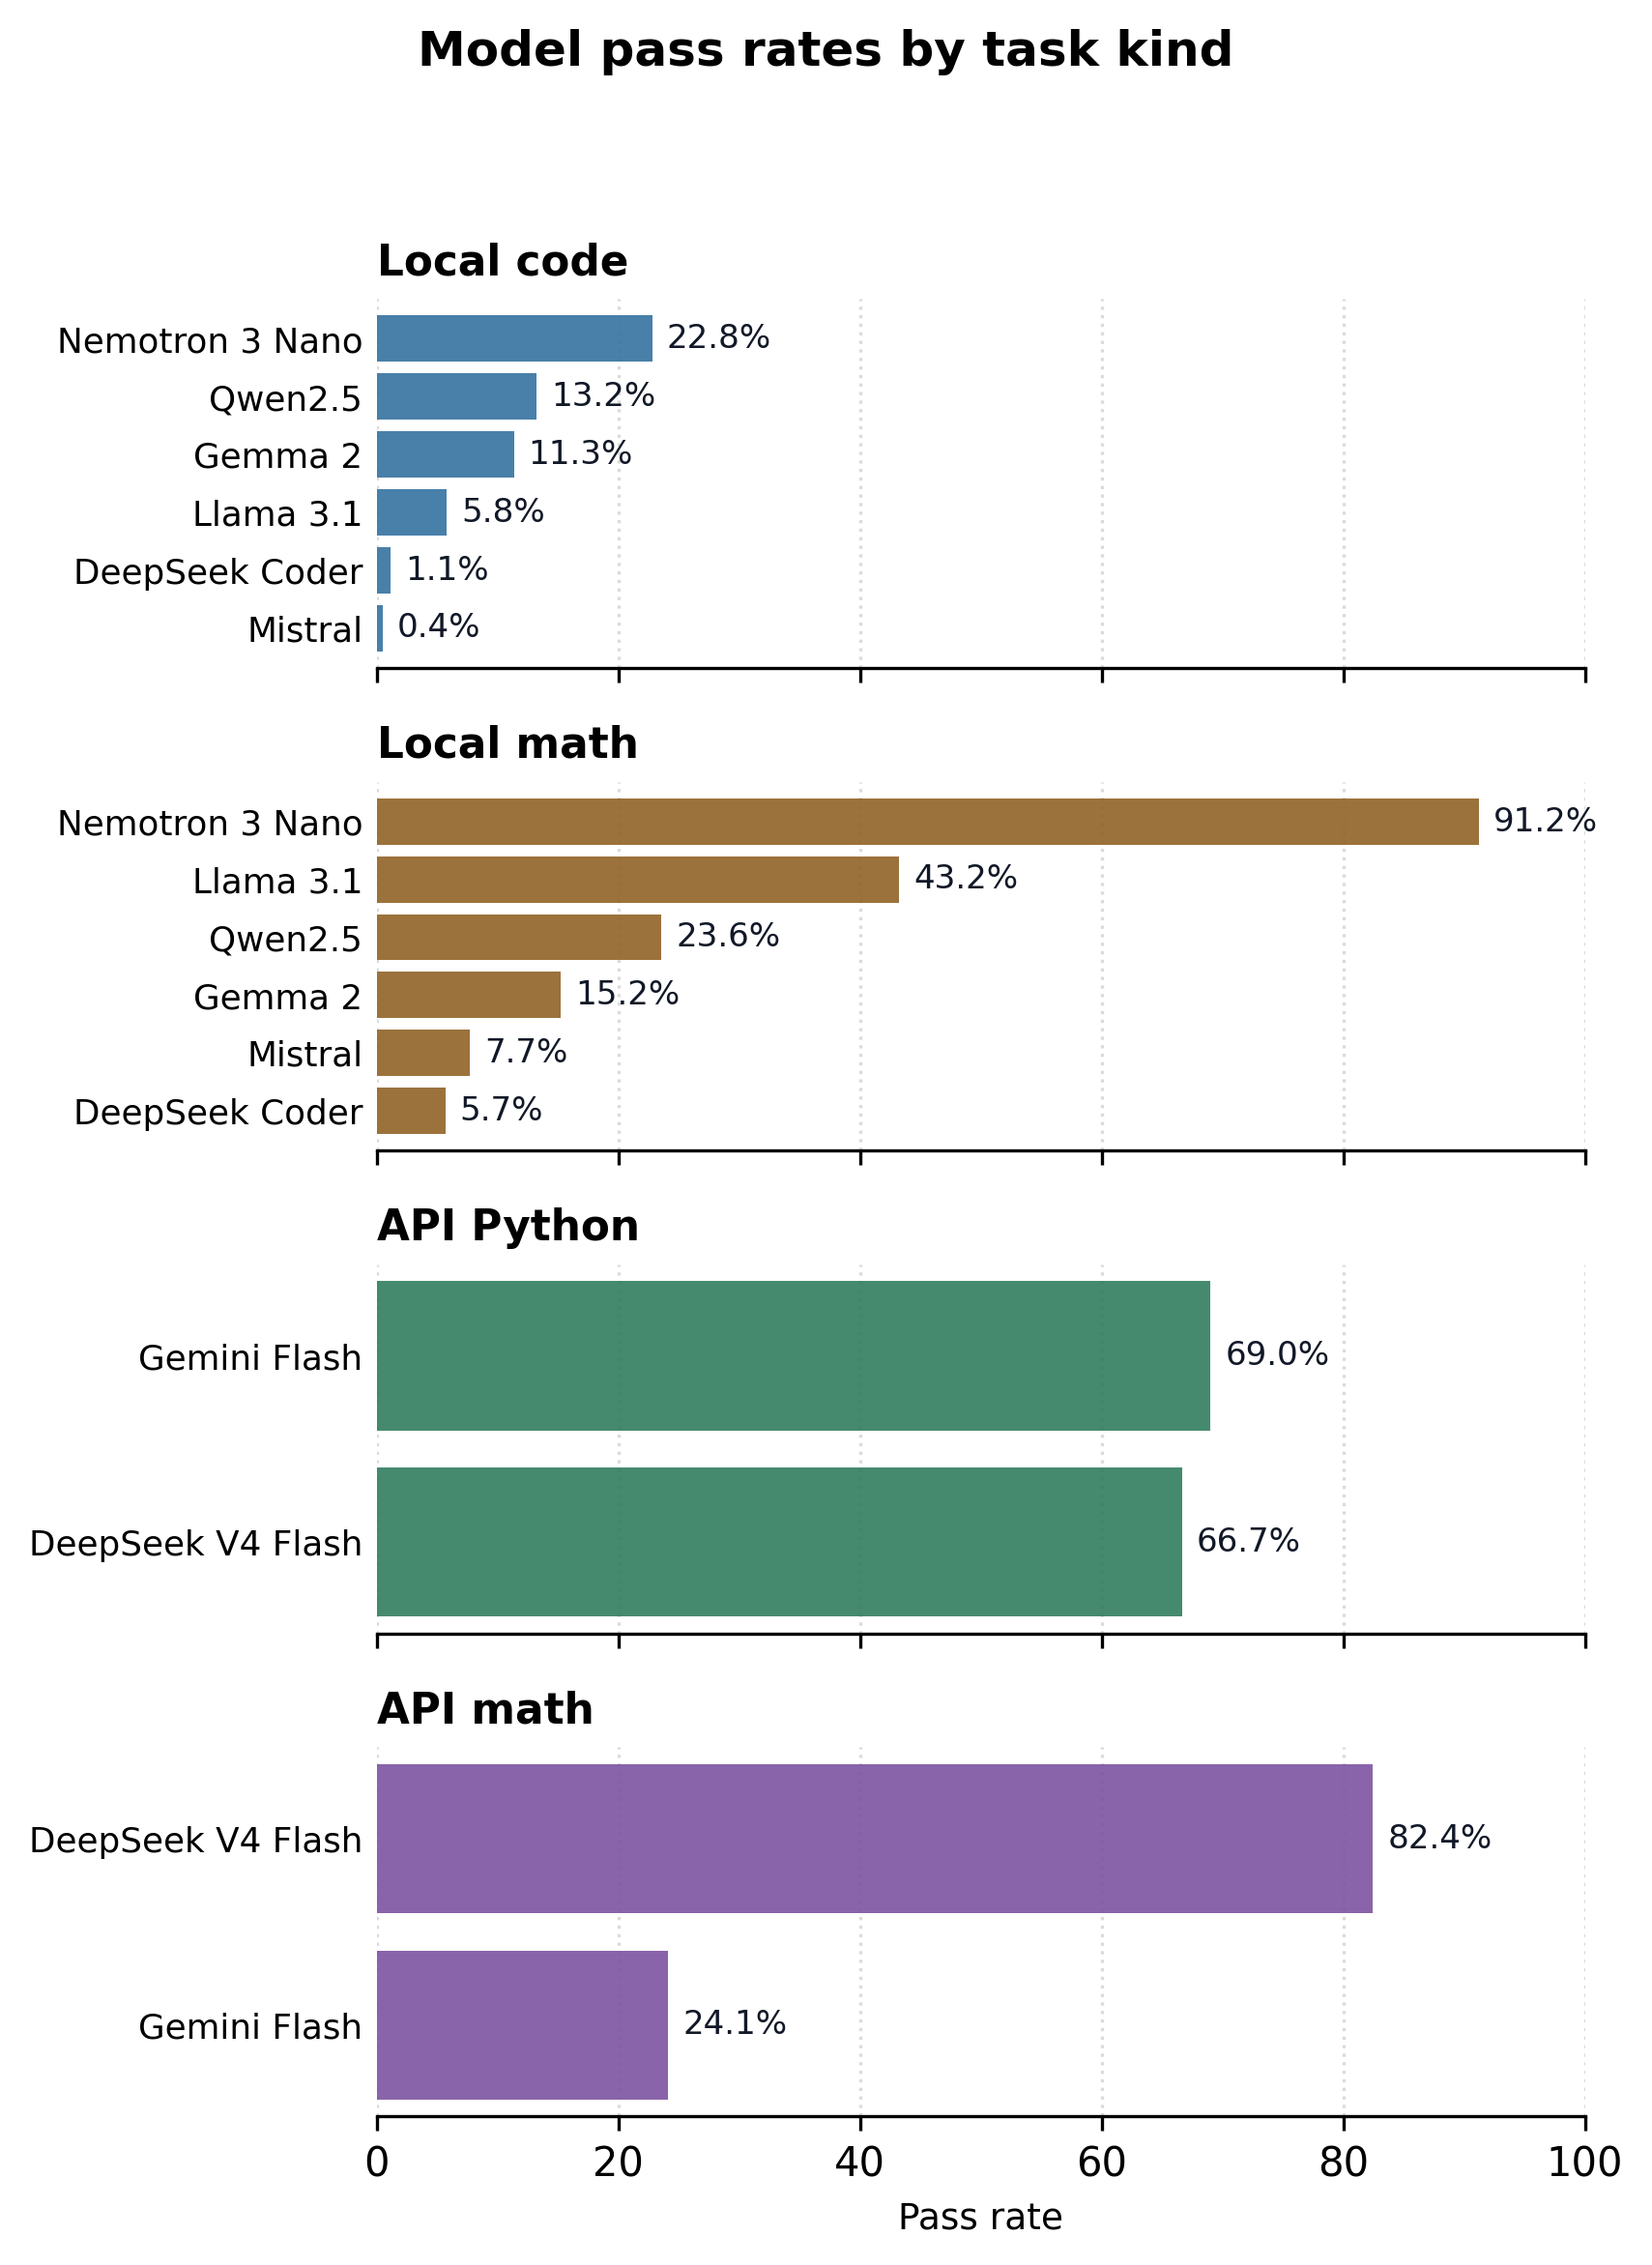
\includegraphics[width=0.95\linewidth,height=\textheight,keepaspectratio,alt={Model pass rates by task kind. The figure highlights that between-model variation is larger than the main prompt-factor effects reported in later sections.}]{figures/model_performance_by_task.png}
\caption{Model pass rates by task kind. The figure highlights that
between-model variation is larger than the main prompt-factor effects
reported in later sections.}
\label{fig:model_performance_by_task}
\end{figure}

\begin{longtable}[]{@{}
  >{\raggedright\arraybackslash}p{(\linewidth - 8\tabcolsep) * \real{0.1667}}
  >{\raggedright\arraybackslash}p{(\linewidth - 8\tabcolsep) * \real{0.1667}}
  >{\raggedleft\arraybackslash}p{(\linewidth - 8\tabcolsep) * \real{0.2222}}
  >{\raggedleft\arraybackslash}p{(\linewidth - 8\tabcolsep) * \real{0.2222}}
  >{\raggedleft\arraybackslash}p{(\linewidth - 8\tabcolsep) * \real{0.2222}}@{}}
\caption{Model-level pass rates and output behavior.}\tabularnewline
\toprule\noalign{}
\begin{minipage}[b]{\linewidth}\raggedright
Task kind
\end{minipage} & \begin{minipage}[b]{\linewidth}\raggedright
Model
\end{minipage} & \begin{minipage}[b]{\linewidth}\raggedleft
Pass rate
\end{minipage} & \begin{minipage}[b]{\linewidth}\raggedleft
Median duration
\end{minipage} & \begin{minipage}[b]{\linewidth}\raggedleft
Mean completion tokens
\end{minipage} \\
\midrule\noalign{}
\endfirsthead
\toprule\noalign{}
\begin{minipage}[b]{\linewidth}\raggedright
Task kind
\end{minipage} & \begin{minipage}[b]{\linewidth}\raggedright
Model
\end{minipage} & \begin{minipage}[b]{\linewidth}\raggedleft
Pass rate
\end{minipage} & \begin{minipage}[b]{\linewidth}\raggedleft
Median duration
\end{minipage} & \begin{minipage}[b]{\linewidth}\raggedleft
Mean completion tokens
\end{minipage} \\
\midrule\noalign{}
\endhead
\bottomrule\noalign{}
\endlastfoot
local code & nemotron-3-nano-4b & 22.8\% & 17.78s & 1646 \\
local code & qwen2.5-7b & 13.2\% & 8.75s & 316 \\
local code & gemma2-9b & 11.3\% & 5.52s & 175 \\
local code & llama3.1-8b & 5.8\% & 11.16s & 394 \\
local code & deepseek-coder-6.7b & 1.1\% & 9.04s & 491 \\
local code & mistral-7b-instruct & 0.4\% & 9.12s & 366 \\
local math & nemotron-3-nano-4b & 91.2\% & 3.15s & 289 \\
local math & llama3.1-8b & 43.2\% & 5.09s & 274 \\
local math & qwen2.5-7b & 23.6\% & 0.68s & 6 \\
local math & gemma2-9b & 15.2\% & 0.80s & 6 \\
local math & mistral-7b-instruct & 7.7\% & 0.89s & 79 \\
local math & deepseek-coder-6.7b & 5.7\% & 5.35s & 287 \\
API Python & gemini-flash & 69.0\% & 10.30s & 359 \\
API Python & deepseek-v4-flash & 66.7\% & 16.12s & 1352 \\
API math & deepseek-v4-flash & 82.4\% & 9.41s & 1127 \\
API math & gemini-flash & 24.1\% & 3.40s & 15 \\
\end{longtable}

The differences between the various models are much greater than the differences between the prompt variants. For instance, the local math gap between Nemotron and DeepSeek Coder is 85.5 percentage points and the greatest pooled local prompt format effect is 4.2 percentage points.

This establishes the scale for the rest of the results: prompt factors are secondary to much larger model and task differences, but still meaningful. A prompt-policy recommendation that ignores the actual model is misleading. The practical question is not whether better prompting can make a weak model perform like a strong one; the evidence does not support that. The useful question is whether better framing makes the chosen model work more smoothly with the evaluator, cost less to run, and fail in fewer predictable ways.

\subsection{Prompt-Factor Effects on Code Tasks}\label{prompt-factor-effects-on-code-tasks}

The pooled results for local code tasks show no significant tone or format effects on correctness. The pass rate for both neutral and aggressive prompts is 9.3\%, while the pass rate for polite prompts is 8.8\%. Role framing reduces the pass rate slightly (from 9.6\% to 8.6\%); the raw pooled contrast is not significant, but the mixed-effects and clustered models both support a small role penalty of about one percentage point. XML shows a slight advantage over plaintext and JSON, but the differences are small and not statistically significant.


\begin{longtable}[]{@{}llrrrr@{}}
\caption{Local code prompt-factor contrasts.}\tabularnewline
\toprule\noalign{}
Factor & Contrast & Pass diff & p & Token diff & Duration diff \\
\midrule\noalign{}
\endfirsthead
\toprule\noalign{}
Factor & Contrast & Pass diff & p & Token diff & Duration diff \\
\midrule\noalign{}
\endhead
\bottomrule\noalign{}
\endlastfoot
tone & aggressive vs neutral & +0.0 pp & 1.000 & +4 & +0.10s \\
tone & polite vs neutral & -0.5 pp & 0.601 & +30 & +0.96s \\
role & role vs none & -1.0 pp & 0.185 & +15 & +0.27s \\
format & JSON vs plaintext & +0.2 pp & 0.860 & -16 & -0.39s \\
format & XML vs plaintext & +0.8 pp & 0.387 & -21 & -0.46s \\
\end{longtable}

For local code tasks, the results are more strongly behavior-based than correctness-based. Completion tokens and duration increase when polite prompts are used, but this does not impact the overall pass rate. Role prompts also increase verbosity. Using JSON/XML decreases the number of tokens and duration while achieving a higher level of result-only/code-only compliance. Ultimately, the behavioral gains driven by prompt usage do not result in meaningful improvements in the pooled pass rate for local code.

In API Python, JSON raises the raw pass rate by 3.2 percentage points while reducing token count by 105 and request time by 1.55 seconds. Similarly, XML raises the pass rate by 4.8 percentage points while reducing tokens by 77 and duration by 1.12 seconds. The raw two-proportion p-values fail to reach the 0.05 significance threshold, but the clustered fixed-effect p-values do. As a result, XML remains statistically significant, while JSON is positive but marginal.

\begin{longtable}[]{@{}llrrrr@{}}
\caption{API Python prompt-format contrasts.}\tabularnewline
\toprule\noalign{}
Factor & Contrast & Pass diff & p & Token diff & Duration diff \\
\midrule\noalign{}
\endfirsthead
\toprule\noalign{}
Factor & Contrast & Pass diff & p & Token diff & Duration diff \\
\midrule\noalign{}
\endhead
\bottomrule\noalign{}
\endlastfoot
format & JSON vs plaintext & +3.2 pp & 0.244 & -105 & -1.55s \\
format & XML vs plaintext & +4.8 pp & 0.074 & -77 & -1.12s \\
\end{longtable}

This comparison has important implications for engineering interpretation. Structured wrappers can assist coding workflows when they enhance parser compatibility and decrease unnecessary output, but this benefit does not apply universally across all model groups or task types.

The API Python result was the strongest positive finding for structured wrappers in the testing, especially when considering the clustered robustness check. This result is also limited to two hosted models, one Python task family, and a very strict code-only system prompt. Consequently, it may be worthwhile to try using JSON or XML wrappers in the coding workflows of API-based development; this will be most beneficial when downstream tooling benefits from compact task boundaries. However, this study does not support applying the same wrapper policy across all model groups or task types.

\subsection{Prompt-Factor Effects on Math Tasks}\label{prompt-factor-effects-on-math-tasks}

Analysis of the data shows that math tasks are more sensitive to prompt framing at the model-specific level than code tasks are. At the local level, using JSON reduces the pooled pass rate by 4.2 percentage points and decreases both tokens used and duration. Using XML reduces the pooled pass rate by 2.2 percentage points, though the unadjusted statistical contrast is not significant. Using role framing also has a positive, but marginal, effect on local math.

\begin{longtable}[]{@{}llrrrr@{}}
\caption{Local math prompt-factor contrasts.}\tabularnewline
\toprule\noalign{}
Factor & Contrast & Pass diff & p & Token diff & Duration diff \\
\midrule\noalign{}
\endfirsthead
\toprule\noalign{}
Factor & Contrast & Pass diff & p & Token diff & Duration diff \\
\midrule\noalign{}
\endhead
\bottomrule\noalign{}
\endlastfoot
tone & aggressive vs neutral & +0.9 pp & 0.539 & +7 & +0.29s \\
tone & polite vs neutral & +1.7 pp & 0.280 & +17 & +0.55s \\
role & role vs none & +2.2 pp & 0.083 & +11 & +0.29s \\
format & JSON vs plaintext & -4.2 pp & 0.007 & -32 & -0.92s \\
format & XML vs plaintext & -2.2 pp & 0.153 & +1 & -0.02s \\
\end{longtable}

Only some models are adversely affected by the local math format effect, as indicated by separate model analyses. Llama 3.1 dropped 15.7 percentage points under JSON and 9.7 percentage points under XML, while DeepSeek Coder dropped 4.3 percentage points under JSON and 5.7 percentage points under XML. The Qwen 2.5 model benefited from role framing, with an increase of 10.2 percentage points. The mixed results indicate that the ultimate conclusion is not that "JSON is bad"; rather, it is that "format effects are model- and task-dependent."

An analysis using the Benjamini-Hochberg correction procedure applied to the 60 local baseline contrasts supports a cautious interpretation of the results. Seven of the 60 have an uncorrected p-value \textless{} 0.05; however, after treating all 60 as one family, only two remain statistically significant: Llama 3.1's JSON penalty in math and Qwen 2.5's role-framing gain in math. When the code and math conditions are treated as two different families of 30 each, there are no remaining significant results for code, but there are 3 significant results for math: Llama 3.1 JSON, Qwen 2.5 role framing, and DeepSeek Coder XML. Therefore, the results of this analysis support the conclusion that sensitivity to prompt types is more of a phenomenon related to the math side of the dataset than the coding side.

For API math, role framing shows a small negative effect: it decreases the pass rate by 2.8 percentage points and increases tokens by 83. The raw comparison is not statistically significant; however, the clustered model check verified that the negative direction remains evident. Because this API pooled result falls outside the corrected model-specific baseline audit and uses only two hosted models, it should be interpreted as an exploratory effect rather than a definite conclusion.

\begin{longtable}[]{@{}llrrrr@{}}
\caption{API math role-framing contrast.}\tabularnewline
\toprule\noalign{}
Factor & Contrast & Pass diff & p & Token diff & Duration diff \\
\midrule\noalign{}
\endfirsthead
\toprule\noalign{}
Factor & Contrast & Pass diff & p & Token diff & Duration diff \\
\midrule\noalign{}
\endhead
\bottomrule\noalign{}
\endlastfoot
role & role vs none & -2.8 pp & 0.238 & +83 & +0.47s \\
\end{longtable}

The combined results show that the math data answers RQ2 and RQ3 more robustly than simply pooling the individual math tables. The direction of format and role effects varies based on the model used and the task type. The math penalties observed with local JSON formatting serve as a cautionary reminder not to assume that structured wrappers will always improve performance. The Qwen role gain and the API role penalty confirm this for persona prompts; that is, framing a question with a role can increase the pass rate, decrease it, or mainly change the verbosity of the output depending on the model and evaluator.

\subsection{Mixed-Effects Inferential Results}\label{mixed-effects-inferential-results}

Table~\ref{tab:mixed-effects-pass} reports the main inferential analysis: mixed-effects logistic models for pass/fail including prompt-factor and model fixed effects and a random intercept per base task, fitted per stratum. The average marginal effects are expressed in percentage points so they can be read alongside the descriptive contrast tables above.

\begin{longtable}[]{@{}llrrr@{}}
\caption{Mixed-effects logistic results for pass/fail by stratum: odds ratios and average marginal effects (AME) in percentage points, with 95\% intervals and posterior p-values.}\label{tab:mixed-effects-pass}\tabularnewline
\toprule\noalign{}
Stratum & Contrast & Odds ratio [95\% int.] & AME pp [95\% int.] & p \\
\midrule\noalign{}
\endfirsthead
\toprule\noalign{}
Stratum & Contrast & Odds ratio [95\% int.] & AME pp [95\% int.] & p \\
\midrule\noalign{}
\endhead
\bottomrule\noalign{}
\endlastfoot
API Python & Aggressive tone & 1.05 [0.83, 1.34] & +0.6 [-2.4, +3.5] & 0.686 \\
API Python & Polite tone & 1.05 [0.83, 1.34] & +0.6 [-2.2, +3.4] & 0.686 \\
API Python & Role framing & 0.92 [0.76, 1.11] & -1.1 [-3.4, +1.2] & 0.381 \\
API Python & JSON wrapper & 1.32 [1.04, 1.68] & +3.4 [+0.4, +6.3] & 0.022 \\
API Python & XML wrapper & 1.55 [1.21, 1.97] & +5.2 [+2.3, +8.2] & \textless{}0.001 \\
API math & Aggressive tone & 1.05 [0.81, 1.38] & +0.5 [-2.0, +3.1] & 0.697 \\
API math & Polite tone & 0.91 [0.70, 1.18] & -0.9 [-3.3, +1.6] & 0.476 \\
API math & Role framing & 0.74 [0.60, 0.92] & -2.8 [-4.8, -0.8] & 0.006 \\
API math & JSON wrapper & 0.87 [0.67, 1.14] & -1.2 [-3.8, +1.4] & 0.325 \\
API math & XML wrapper & 0.78 [0.60, 1.02] & -2.3 [-4.9, +0.1] & 0.069 \\
Local code & Aggressive tone & 0.98 [0.80, 1.20] & -0.1 [-1.0, +0.9] & 0.858 \\
Local code & Polite tone & 0.89 [0.72, 1.09] & -0.5 [-1.4, +0.4] & 0.265 \\
Local code & Role framing & 0.81 [0.68, 0.96] & -1.0 [-1.7, -0.2] & 0.013 \\
Local code & JSON wrapper & 1.01 [0.83, 1.24] & +0.1 [-0.8, +1.1] & 0.900 \\
Local code & XML wrapper & 1.15 [0.94, 1.41] & +0.7 [-0.3, +1.6] & 0.164 \\
Local math & Aggressive tone & 1.11 [0.95, 1.29] & +0.9 [-0.5, +2.3] & 0.198 \\
Local math & Polite tone & 1.20 [1.03, 1.40] & +1.6 [+0.2, +3.0] & 0.019 \\
Local math & Role framing & 1.28 [1.13, 1.45] & +2.1 [+1.0, +3.2] & \textless{}0.001 \\
Local math & JSON wrapper & 0.62 [0.52, 0.72] & -4.1 [-5.4, -2.7] & \textless{}0.001 \\
Local math & XML wrapper & 0.78 [0.66, 0.91] & -2.2 [-3.4, -0.8] & 0.001 \\
\end{longtable}

According to the mixed-effects results, all of the headline findings are confirmed. The results of the main inferential analysis confirm the benefit of the structured format in API Python code for both JSON (OR 1.32, p = 0.022) and XML (OR 1.55, p \textless{} 0.001). The penalty for local math in JSON is clearly established (OR 0.62, p \textless{} 0.001); the penalty for local math in XML is also confirmed (OR 0.78, p = 0.001), as are the gain from local math in role-framing (OR 1.28, p \textless{} 0.001) and the small polite-tone gain in local math (OR 1.20, p = 0.019). The role-framing penalty in API math code, which was regarded as exploratory in the descriptive analysis, was confirmed in the mixed model (OR 0.74, p = 0.006). The small penalty for the local-code role is also confirmed in the mixed analysis (OR 0.81, p = 0.013); however, at roughly one percentage point, it remains practically minor. No tone effects can be regarded as significant when analyzing any code format.

The behavioral mixed models present the same findings as the descriptive behavior tables. Using linear mixed models with random task-specific intercepts, polite language leads to an increase in log completion tokens and log duration in the local strata, while the use of both JSON and XML decreases these figures; additionally, role framing modestly increases them. These overall effect directions confirm what is seen in the descriptive behavior tables. Furthermore, the result-only compliance outcome remains constant for API code under strict system prompts, meaning no compliance model can be estimated in that context.

\subsection{Output Behavior: Tokens, Duration, and Result-Only Compliance}\label{output-behavior-tokens-duration-and-result-only-compliance}

Prompt framing changes observable output behavior more reliably than
correctness. In the case of coding tasks, a polite tone leads to 12.40\% more completion tokens, a 7.00-percentage-point decline in result-only compliance, and an increase of 10.76\% in duration. Role framing results in 3.17\% more tokens and 2.41\% longer duration. JSON and XML reduce tokens and duration but improve result-only compliance.

Figure~\ref{fig:behavior-effects} visualizes these behavior effects, split by unit: panel (a) shows token and duration effects in percent, panel (b) shows result-only compliance effects in percentage points. The largest behavior changes
are not always correctness gains: polite tone increases output length
and duration, while JSON strongly shortens local math responses.

\begin{figure}
\centering
\begin{minipage}[b]{0.78\linewidth}
\centering
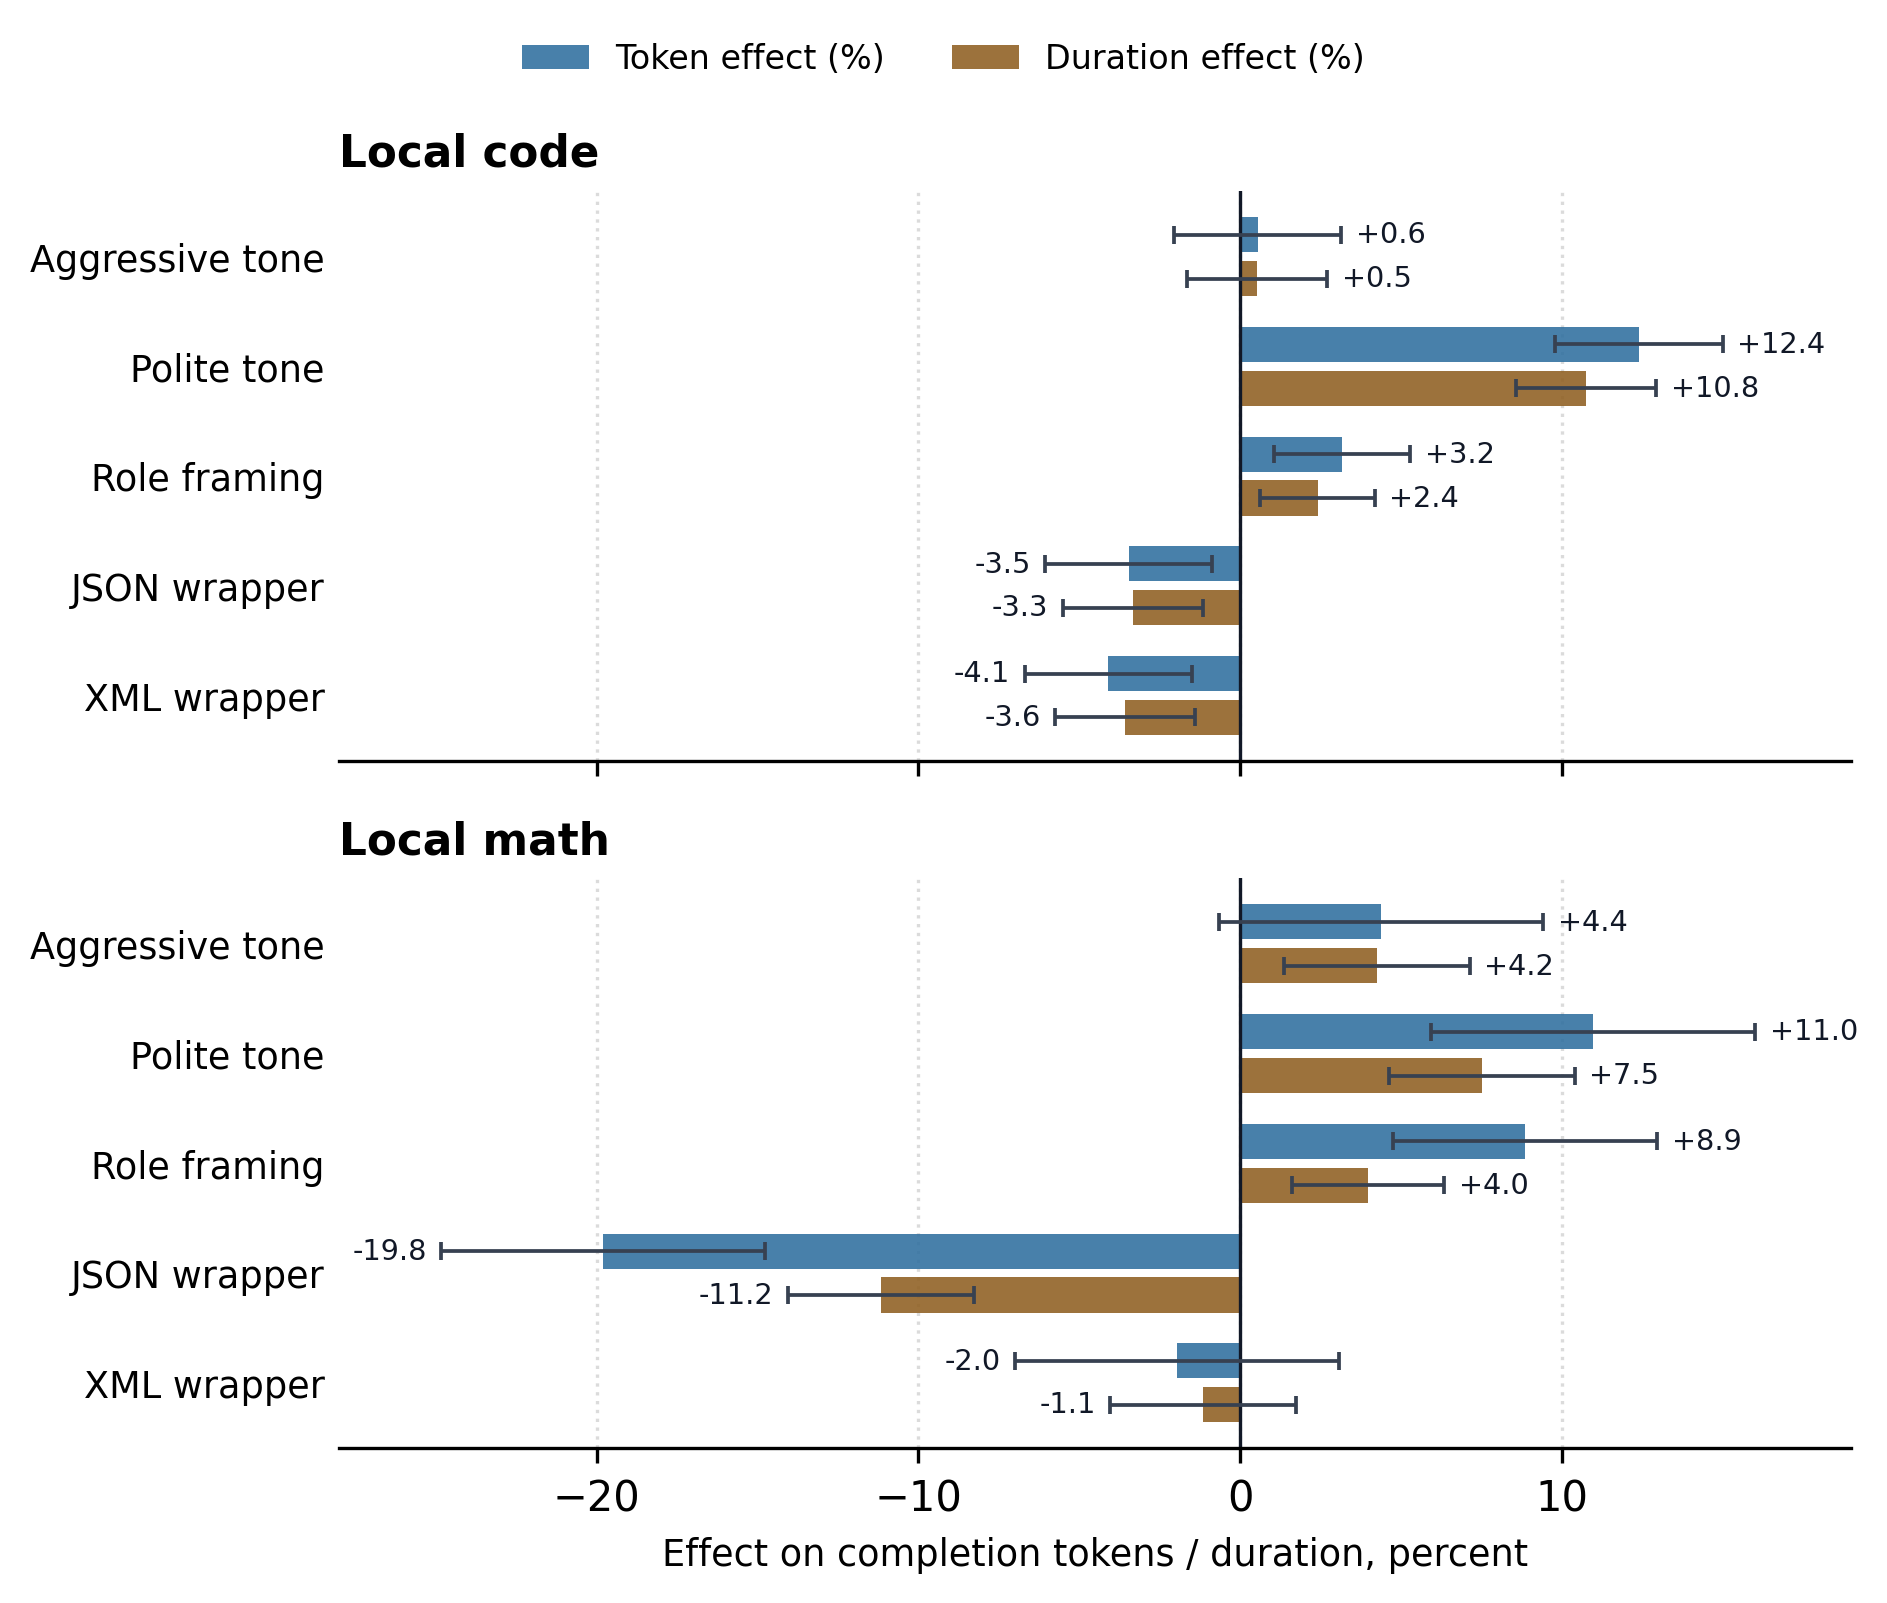
\includegraphics[width=\linewidth,alt={Token and duration effects in percent for local code and local math.}]{figures/behavior_effects_tokens_duration.png}
\centering\textbf{(a)} Token and duration effects, percent
\end{minipage}

\vspace{0.8em}

\begin{minipage}[b]{0.78\linewidth}
\centering
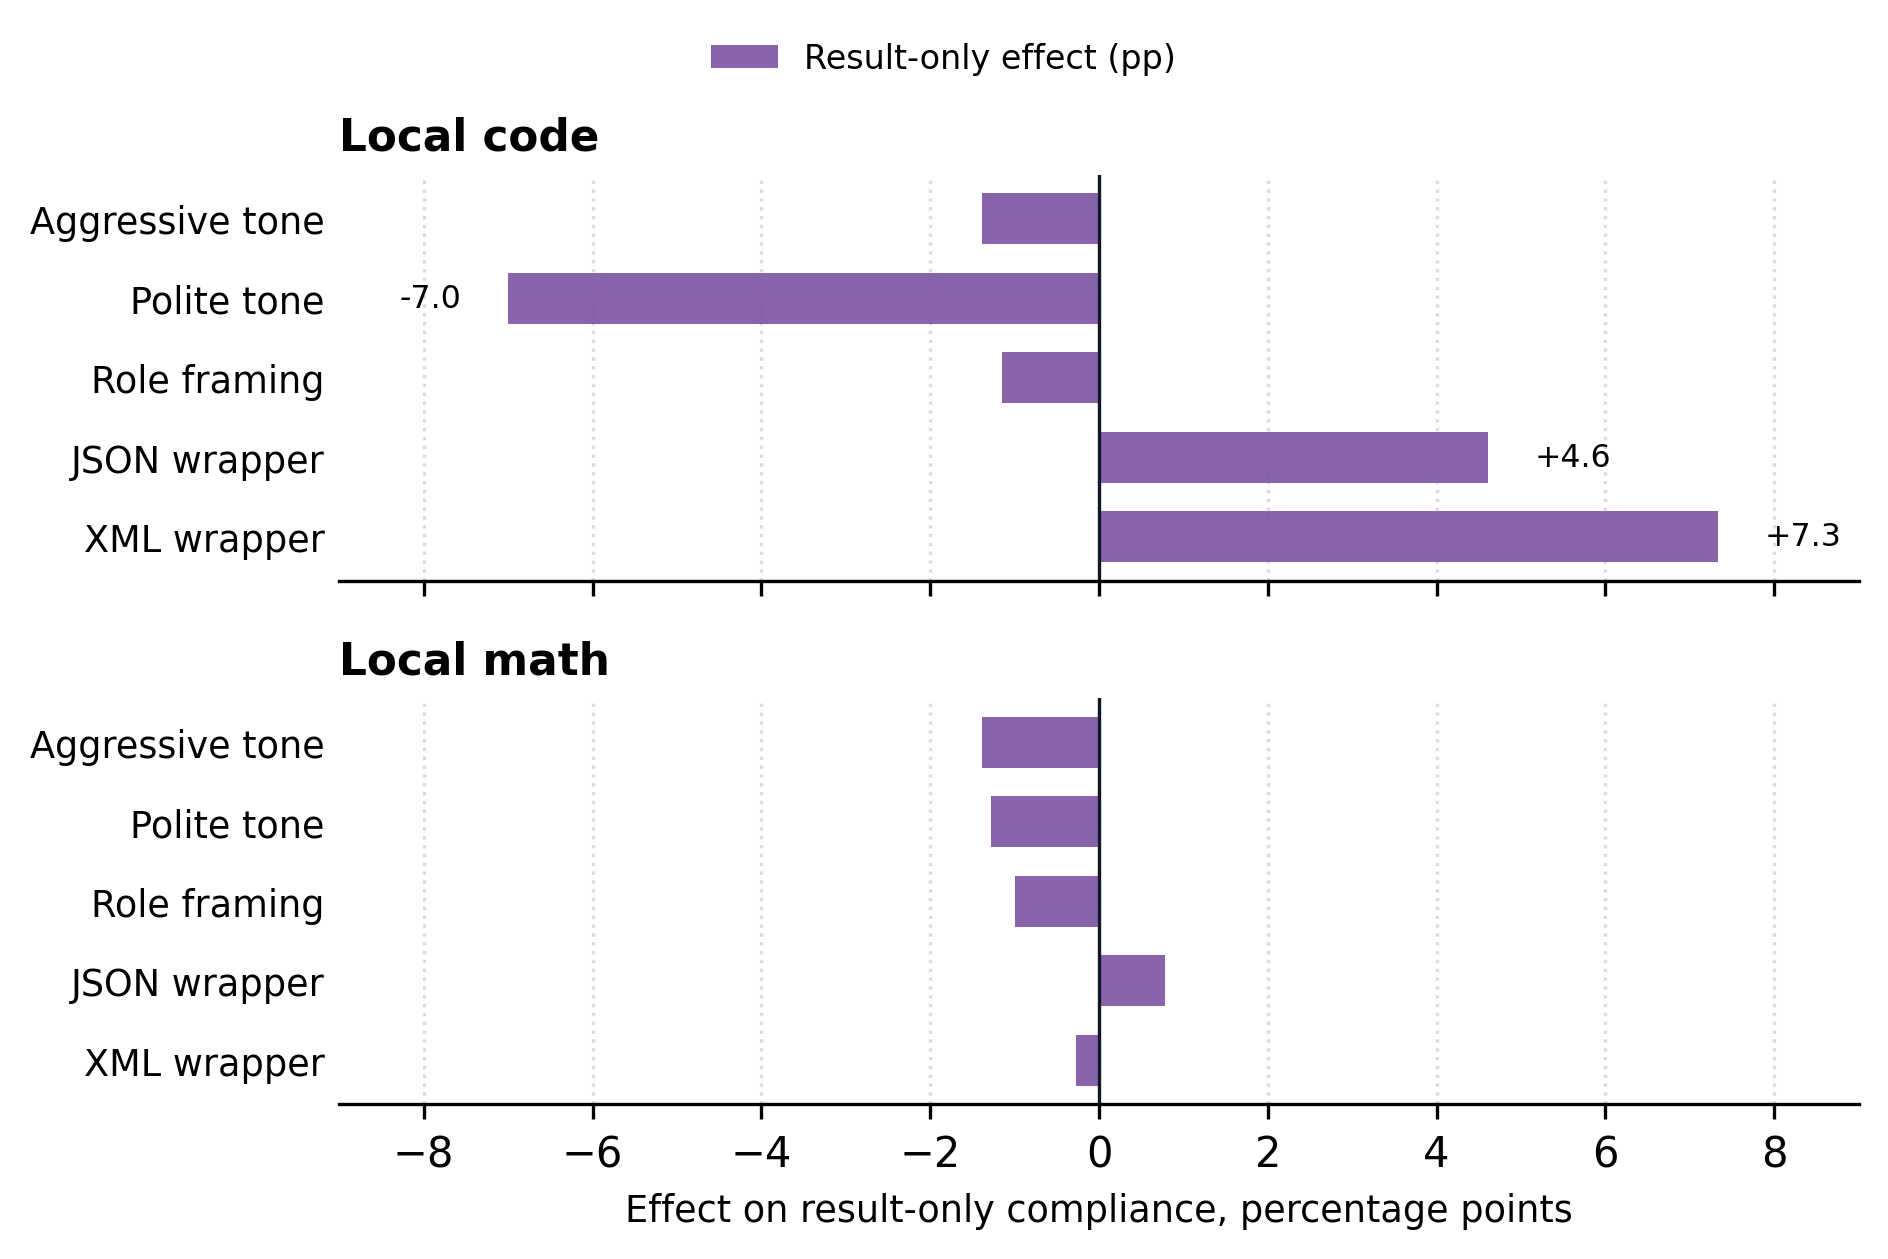
\includegraphics[width=\linewidth,alt={Result-only compliance effects in percentage points for local code and local math.}]{figures/behavior_effects_compliance.png}
\centering\textbf{(b)} Result-only compliance effects, percentage points
\end{minipage}
\caption{Prompt-factor effects on output behavior for local code and
local math. Panel (a): effects on completion tokens and duration, in
percent. Panel (b): effects on result-only compliance, in percentage
points.}
\label{fig:behavior-effects}
\end{figure}

\begin{longtable}[]{@{}
  >{\raggedright\arraybackslash}p{(\linewidth - 6\tabcolsep) * \real{0.2000}}
  >{\raggedleft\arraybackslash}p{(\linewidth - 6\tabcolsep) * \real{0.2667}}
  >{\raggedleft\arraybackslash}p{(\linewidth - 6\tabcolsep) * \real{0.2667}}
  >{\raggedleft\arraybackslash}p{(\linewidth - 6\tabcolsep) * \real{0.2667}}@{}}
\caption{Local code behavior effects.}\tabularnewline
\toprule\noalign{}
\begin{minipage}[b]{\linewidth}\raggedright
Local code factor
\end{minipage} & \begin{minipage}[b]{\linewidth}\raggedleft
Token effect
\end{minipage} & \begin{minipage}[b]{\linewidth}\raggedleft
Result-only effect
\end{minipage} & \begin{minipage}[b]{\linewidth}\raggedleft
Duration effect
\end{minipage} \\
\midrule\noalign{}
\endfirsthead
\toprule\noalign{}
\begin{minipage}[b]{\linewidth}\raggedright
Local code factor
\end{minipage} & \begin{minipage}[b]{\linewidth}\raggedleft
Token effect
\end{minipage} & \begin{minipage}[b]{\linewidth}\raggedleft
Result-only effect
\end{minipage} & \begin{minipage}[b]{\linewidth}\raggedleft
Duration effect
\end{minipage} \\
\midrule\noalign{}
\endhead
\bottomrule\noalign{}
\endlastfoot
Aggressive tone & +0.55\% & -1.39 pp & +0.52\% \\
Polite tone & +12.40\% & -7.00 pp & +10.76\% \\
Role framing & +3.17\% & -1.15 pp & +2.41\% \\
JSON wrapper & -3.46\% & +4.61 pp & -3.32\% \\
XML wrapper & -4.10\% & +7.33 pp & -3.57\% \\
\end{longtable}

In math tasks, polite prompts increase tokens and duration, and role prompts do the same, but JSON strongly reduces both. Result-only compliance is also relatively unchanged for math tasks because the majority of models have stable response patterns regardless of the prompt. Typically, Qwen, Gemma, and Nemotron provide short responses, whereas Llama and DeepSeek provide lengthy responses.

\begin{longtable}[]{@{}
  >{\raggedright\arraybackslash}p{(\linewidth - 6\tabcolsep) * \real{0.2000}}
  >{\raggedleft\arraybackslash}p{(\linewidth - 6\tabcolsep) * \real{0.2667}}
  >{\raggedleft\arraybackslash}p{(\linewidth - 6\tabcolsep) * \real{0.2667}}
  >{\raggedleft\arraybackslash}p{(\linewidth - 6\tabcolsep) * \real{0.2667}}@{}}
\caption{Local math behavior effects.}\tabularnewline
\toprule\noalign{}
\begin{minipage}[b]{\linewidth}\raggedright
Local math factor
\end{minipage} & \begin{minipage}[b]{\linewidth}\raggedleft
Token effect
\end{minipage} & \begin{minipage}[b]{\linewidth}\raggedleft
Result-only effect
\end{minipage} & \begin{minipage}[b]{\linewidth}\raggedleft
Duration effect
\end{minipage} \\
\midrule\noalign{}
\endfirsthead
\toprule\noalign{}
\begin{minipage}[b]{\linewidth}\raggedright
Local math factor
\end{minipage} & \begin{minipage}[b]{\linewidth}\raggedleft
Token effect
\end{minipage} & \begin{minipage}[b]{\linewidth}\raggedleft
Result-only effect
\end{minipage} & \begin{minipage}[b]{\linewidth}\raggedleft
Duration effect
\end{minipage} \\
\midrule\noalign{}
\endhead
\bottomrule\noalign{}
\endlastfoot
Aggressive tone & +4.39\% & -1.39 pp & +4.24\% \\
Polite tone & +10.97\% & -1.28 pp & +7.51\% \\
Role framing & +8.86\% & -1.00 pp & +3.98\% \\
JSON wrapper & -19.80\% & +0.78 pp & -11.16\% \\
XML wrapper & -1.96\% & -0.28 pp & -1.14\% \\
\end{longtable}

Behavioral impacts are significant to applied systems. Even when the level of correctness doesn’t change, a particular prompt may increase costs, latency, and parsing difficulty. On the other hand, a prompt can make the output easier for a parser to process, even if the model’s actual performance on the task does not improve.

This is the clearest answer to our third research question. Prompt framing changes how models answer more reliably than it changes whether answers are correct. In coding tasks, this distinction is critical from an operations perspective, since excessive verbosity or a lack of clear delimiters in the response will prevent the answer from being automatically extracted. In mathematics tasks, this distinction manifests differently: many models already provide very short numerical outputs, leaving less room for behavioral variations, though changes in token count or time will still signal different response strategies. Reporting both behavioral and correctness information in tandem will help prevent an efficiency gain from being confused with a quality gain.


\subsection{Mediation and Behavioral-Control Results}\label{mediation-and-behavioral-control-results}

The mediation-style analysis investigates how much of each prompt effect remains after adjustment for observable behavior. For code tasks, the descriptive polite-tone contrast is an overall 0.50 percentage-point decrease in pass rate. After adjustment for tokens, result-only compliance, and duration, the coefficient is attenuated and shifts to a positive 0.17 percentage points. In other words, the apparent polite-tone penalty in code generation is associated with the measured behavioral variables: polite prompts are associated with longer, slower, and less parseable outputs, and once those behaviors are adjusted for, no negative correctness contrast remains. Because the adjustment variables are post-treatment, this pattern is consistent with a verbosity/parser pathway but does not prove it.

The total prompt-factor correctness contrasts and the coefficients after adjustment for measured behavioral variables are shown in Figure ~\ref{fig:mediation-controls}. The code-task effects are small before and after adjustment. For the math tasks, the JSON coefficient is also attenuated after adjustment but remains negative; reduced verbosity is therefore associated with part of the local-math drop, but not all of it.

\begin{figure}
\centering
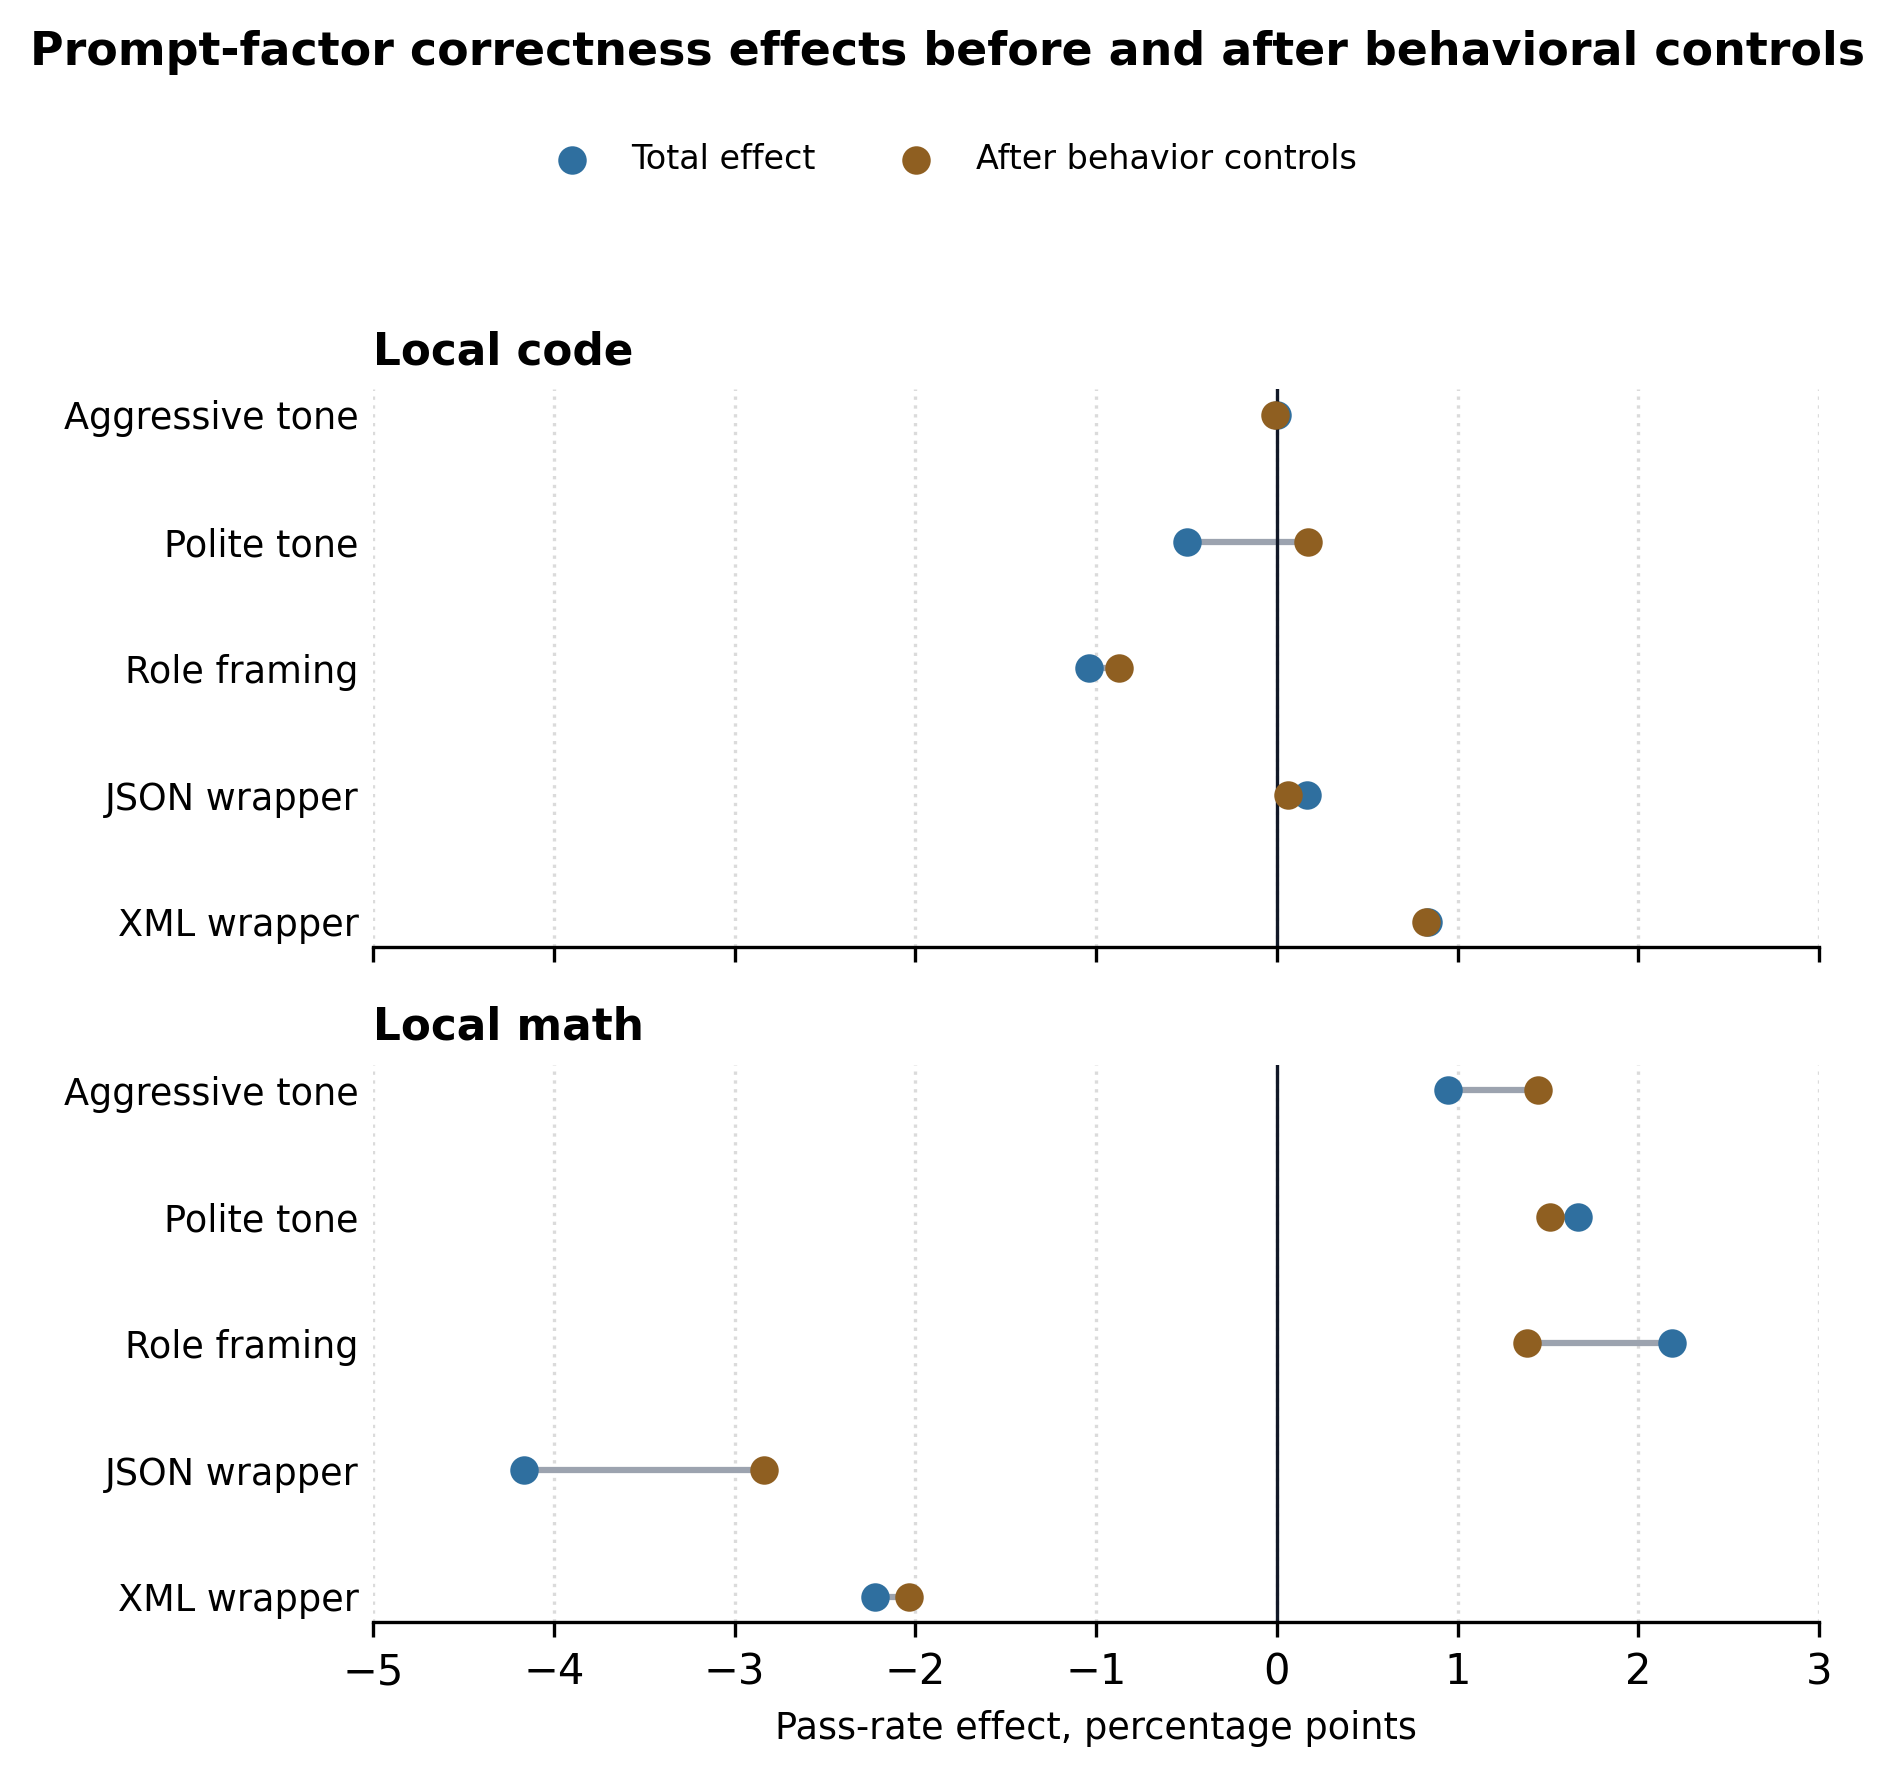
\includegraphics[width=0.95\linewidth,height=\textheight,keepaspectratio,alt={Prompt-factor correctness effects before and after controlling for completion tokens, result-only compliance, and duration.}]{figures/mediation_controls.png}
\caption{Prompt-factor correctness effects before and after controlling
for completion tokens, result-only compliance, and duration.}
\label{fig:mediation-controls}
\end{figure}

\begin{longtable}[]{@{}lrr@{}}
\caption{Local code correctness contrasts before and after adjustment
for measured behavioral variables.}\tabularnewline
\toprule\noalign{}
Local code factor & Total contrast & After behavioral adjustment \\
\midrule\noalign{}
\endfirsthead
\toprule\noalign{}
Local code factor & Total contrast & After behavioral adjustment \\
\midrule\noalign{}
\endhead
\bottomrule\noalign{}
\endlastfoot
Aggressive tone & -0.00 pp & -0.01 pp \\
Polite tone & -0.50 pp & +0.17 pp \\
Role framing & -1.04 pp & -0.87 pp \\
JSON wrapper & +0.17 pp & +0.06 pp \\
XML wrapper & +0.83 pp & +0.82 pp \\
\end{longtable}

For math tasks, the JSON coefficient remains negative after adjustment. The total contrast is -4.17 percentage points; after adjustment for token amount, result-only compliance, and duration, the remaining coefficient is -2.84 percentage points. The measured behaviors are therefore associated with part of the observed contrast, but not all of it. This pattern indicates that JSON-style framing is associated with both the model's observable behavior and downstream correctness in this setting; it should not be interpreted as evidence about the model's hidden reasoning processes.

\begin{longtable}[]{@{}lrr@{}}
\caption{Local math correctness contrasts before and after adjustment
for measured behavioral variables.}\tabularnewline
\toprule\noalign{}
Local math factor & Total contrast & After behavioral adjustment \\
\midrule\noalign{}
\endfirsthead
\toprule\noalign{}
Local math factor & Total contrast & After behavioral adjustment \\
\midrule\noalign{}
\endhead
\bottomrule\noalign{}
\endlastfoot
Aggressive tone & +0.94 pp & +1.45 pp \\
Polite tone & +1.67 pp & +1.51 pp \\
Role framing & +2.19 pp & +1.38 pp \\
JSON wrapper & -4.17 pp & -2.84 pp \\
XML wrapper & -2.22 pp & -2.04 pp \\
\end{longtable}

Thus, the mediation-style tables serve primarily as associational checkpoints and should not be viewed as a replacement for correctness results or as proof of a mechanism. For local code, the attenuated tone and role coefficients are consistent with a pipeline explanation in which tone and role framing mainly relate to verbosity and ease of parsing. For local math, the measured behavior variables account for only part of the JSON penalty. This residual negative coefficient should be viewed with caution; however, it is exactly the type of outcome that justifies validating prompt policies per task and model rather than trusting universal advice.

\subsection{Clustered Linear-Probability Robustness Check}\label{clustered-linear-probability-robustness-check}

As a robustness check on the mixed-effects results, we fit pass/fail linear probability models separately by model group and task type, with prompt factors and model fixed effects and standard errors clustered by base task. The clustered LPM addresses the same repeated-task dependence as the mixed model with a different set of assumptions, and it does not deviate significantly from the main results while correcting for the repetition of the same 50 base tasks across all prompt variants and models.

In the clustered analysis, the core direction of headline effects remains stable and agrees with the mixed-effects model. For API Python, XML stays significant at +4.83 percentage points (clustered SE 1.77, p=0.006), while JSON is positive but marginal at +3.17 percentage points (clustered SE 1.73, p=0.068). For local math, JSON stands at -4.17 percentage points (clustered SE 1.11, p \textless{} 0.001) and XML remains negative at -2.22 percentage points (clustered SE 1.02, p=0.030). Local math role framing is positive at +2.19 percentage points (clustered SE 0.69, p=0.002), and polite tone is also positive at +1.67 percentage points (clustered SE 0.79, p=0.035).

The clustered check sharpens the key narrative instead of reversing it. For positive results, the most robust format is API Python XML, while the most robust negative format is local math JSON. Every effect that is significant in the mixed-effects model is directionally consistent in the clustered LPM, and the remaining effects are either small, model-dependent, or exploratory.

\subsection{Dominant-Model Sensitivity and Aggregation Risk}\label{dominant-model-sensitivity-and-aggregation-risk}

A single dominant model can overshadow the pooled averages. Removing Nemotron leads to a drop in the local math pass rate from 31.1\% to 19.1\%. The API math pass rate drops by almost half, from 53.3\% to 24.1\%, when DeepSeek V4 Flash is removed. API Python is more stable because Gemini Flash has a similar Python pass rate to DeepSeek V4 Flash.

\begin{longtable}[]{@{}llrr@{}}
\caption{Dominant-model sensitivity of pooled pass rates.}\tabularnewline
\toprule\noalign{}
Sensitivity dataset & Task kind & Full avg. & Without dominant \\
\midrule\noalign{}
\endfirsthead
\toprule\noalign{}
Sensitivity dataset & Task kind & Full avg. & Without dominant \\
\midrule\noalign{}
\endhead
\bottomrule\noalign{}
\endlastfoot
Local, no Nemotron & code & 9.1\% & 6.4\% \\
Local, no Nemotron & math & 31.1\% & 19.1\% \\
API, no DeepSeek & math & 53.3\% & 24.1\% \\
API, no DeepSeek & python & 67.8\% & 69.0\% \\
\end{longtable}

Pass-rate averages, however, do not show whether the prompt effects themselves are distorted by the dominant model. We therefore re-estimated every main tone, role, and format contrast with and without the dominant model in each group, using both the clustered LPM and the mixed-effects logistic model. Table~\ref{tab:dominant-effects} reports the percentage-point effects in both panels; for the API group, the leave-one-out panel contains only Gemini Flash, so those columns are single-model estimates.

\begin{longtable}[]{@{}llrrrr@{}}
\caption{Prompt-factor effects with and without the dominant model: clustered-LPM percentage-point contrasts and mixed-effects average marginal effects (AME pp).}\label{tab:dominant-effects}\tabularnewline
\toprule\noalign{}
Stratum & Contrast & LPM full & LPM w/o dom. & AME full & AME w/o dom. \\
\midrule\noalign{}
\endfirsthead
\toprule\noalign{}
Stratum & Contrast & LPM full & LPM w/o dom. & AME full & AME w/o dom. \\
\midrule\noalign{}
\endhead
\bottomrule\noalign{}
\endlastfoot
API Python & JSON wrapper & +3.2 & +1.3 & +3.4 & +1.6 \\
API Python & XML wrapper & +4.8 & +2.7 & +5.2 & +3.1 \\
API math & Role framing & -2.8 & -2.4 & -2.8 & -4.1 \\
API math & JSON wrapper & -1.3 & -3.7 & -1.2 & -6.1 \\
API math & XML wrapper & -2.3 & -0.0 & -2.3 & -0.2 \\
Local code & Role framing & -1.0 & -0.9 & -1.0 & -0.9 \\
Local math & Polite tone & +1.7 & +2.3 & +1.6 & +2.3 \\
Local math & Role framing & +2.2 & +2.4 & +2.1 & +2.3 \\
Local math & JSON wrapper & -4.2 & -5.3 & -4.1 & -5.2 \\
Local math & XML wrapper & -2.2 & -2.5 & -2.2 & -2.4 \\
\end{longtable}

The re-estimation indicate that the local prompt effects are not merely an artifact of Nemotron's dominance. In the absence of Nemotron, the local math JSON penalty has a slightly greater impact (-5.2 pp AME compared to -4.1 pp in the full panel) while still being highly statistically significant, and the two local math prompt gains (role framing and politeness) exhibit no observable change in their magnitude. Finally, even the small local-code role penalty is just as consistent between both estimates (-0.9 pp AME). Overall, while the leading local model shifts the pooled pass rate by 12 points, it leaves the prompt-effect estimates intact in both direction and magnitude.

The API group displays a different pattern, as expected in a two-model panel. The benefit of the API Python structured format shrinks with the removal of DeepSeek V4 Flash, causing the XML effect to fall from +5.2 to +3.1 pp AME and the JSON effect to decrease from +3.4 to +1.6 pp AME, and neither is shown to be statistically significant in a Gemini-only panel. Therefore, the combined API Python effect must be interpreted as a two-model average with the major input from DeepSeek, and not a feature attributable to each model. The API math role-framing penalty, on the contrary, still holds and becomes even greater in the Gemini-only panel (-4.1 pp AME), which means that it is not influenced only by DeepSeek. The API math XML penalty does not remain after the removal (-0.2 pp AME), thus emphasizing its exploratory character.

This sensitivity test lends support to the primary methodological point: that prompt-policy conclusions must not come from pooled averages only, but be derived from each model group and task type, with the dominant-model dependence of each effect stated explicitly.

Given the unusually high local math pass rate of 91.2\%, Nemotron underwent an independent repository audit. The audited Nemotron math file consists of 900 distinct runs, balanced across 50 base tasks and 18 prompt variants, with zero duplicate task IDs. Since re-computing the pass/fail scores using \texttt{expected\_answer} and \texttt{extracted\_values} reproduced 821 out of 900 passes with zero mismatches against the stored \texttt{passed} field, and a scan found no expected-answer leakage, it is fair to say that the high score is stable across each prompt variant. This figure further demonstrates that the value in question can be treated as a real result, thus justifying the no-Nemotron sensitivity check.

To illuminate the 91.2\% figure at the task level, we provide a breakdown of how the 50 local math tasks perform across the 18 different prompt conditions tested by Nemotron. As shown in Table~\ref{tab:nemotron-task-summary}, the high pass rate is not due to just a few lucky task variants; 42 of the 50 tasks pass in all 18 conditions, 6 tasks pass under some conditions, and only 2 tasks fail in all conditions. Thus, the high average reflects a model that consistently solves most of the task set across various framing conditions, rather than being a mere evaluation artifact affecting a small number of conditions.

\begin{longtable}[]{@{}lr@{}}
\caption{Nemotron 3 Nano local math: task-level solve pattern across the 18 prompt conditions (50 base tasks).}\label{tab:nemotron-task-summary}\tabularnewline
\toprule\noalign{}
Solve pattern across 18 prompt conditions & Number of tasks (of 50) \\
\midrule\noalign{}
\endfirsthead
\toprule\noalign{}
Solve pattern across 18 prompt conditions & Number of tasks (of 50) \\
\midrule\noalign{}
\endhead
\bottomrule\noalign{}
\endlastfoot
Solved under all 18 conditions & 42 \\
Solved under some conditions (1--17) & 6 \\
Solved under no condition & 2 \\
\end{longtable}

\subsection{Error and Failure Modes}\label{error-and-failure-modes}

The experiment shows some of the possible failure modes. Regarding code-based tasks, a few of these failures include wrong algorithms, mistakes in syntax, missing functions, or even outputs incorporating prose or markdown that the extractor cannot cleanly process. The use of both polite and role prompts may lead to parsing issues since they can lead to more explanatory text. Formats such as JSON and XML may make outputs more compact, but they do not guarantee correctness.

The types of failures in math tasks include wrong answers, missing final-answer markers, too brief or vague answers, and extraction ambiguity. Using JSON reduces the duration and length of local math responses while decreasing the pass rate, suggesting that using compact formatting can lower accuracy in certain reasoning tasks even if the requested output is final-result-only. This does not mean that showing reasoning is always required; rather, the results show that less verbose responses are associated with lower local math accuracy in this study.

Representative cases demonstrate the contrast between task-related failures and parser or interface failures. In one Nemotron code run, the response returned by the model was empty, leading to the evaluation of \texttt{No code extracted}. In a different incident with Qwen 2.5, Python code was executed; however, the model used helper names that did not satisfy the requirements of the callable interface, due to which the code execution failed with name-resolution errors. One more instance occurred when a local math run was conducted in Qwen 2.5 using the JSON-format prompt. The result was that the answer \texttt{6} was given when the expected answer was \texttt{12}, showing the compact nature of the answer, which was easily extractable yet erroneous. These examples support the broader interpretation that correctness, extraction compatibility, and output behavior should be reported separately.

\section{Discussion}
\subsection{Main Interpretation}\label{main-interpretation}

The primary interpretation is balanced. Prompt framing is not a universal accuracy tool, but it is a real engineering variable: model ability dominates correctness, while prompt choices change output form, parseability, latency, cost, and sometimes correctness. Prompts must therefore be evaluated as part of the overall LLM system, not adopted as universal rules.

Prompt effects are also better understood as interface effects between model and evaluator than as changes in model competence. Polite code prompts increase explanatory language, which makes extraction harder, while structured wrappers reduce verbosity. In local math tasks, the compactness induced by some prompt formats is associated with lower answer accuracy. The practical lesson is that prompts, parsers, validators, and task definitions form one measurement system.

\subsection{Implications for LLM-Based Coding Systems}\label{implications-for-llm-based-coding-systems}

Reliable coding assistants need engineering beyond prompt design: explicit output contracts and automated validation. Workflows should separate reasoning from the final artifact, produce a clean code artifact at the end, and avoid relying on prompt tricks like politeness or role labeling for correctness.

The API Python results show the value of structured wrappers in some coding workflows: raw pass-rate contrasts improve under JSON and XML while tokens and duration decrease, and the mixed-effects model supports both effects. This suggests that structured wrappers can improve compatibility with automated evaluation when they align with the task and model. The local math result shows the danger of turning this into universal advice.

The same principle applies to agentic workflows, where model outputs are consumed by downstream systems. A response that provides human-friendly explanations may be unusable to automated tools due to extra commentary or formatting inconsistencies, while machine-friendly output may be too terse for human debugging. Prompt policy must therefore be directed at the actual output consumer: the instruction should state the required artifact, the evaluator should accept common valid forms, and systems serving both human and automated consumers should separate these phases rather than asking one prompt to satisfy incompatible goals.

\subsection{Why Code and Math Differ}\label{why-code-and-math-differ}

Programming and mathematical evaluations impose different requirements for output results. Code evaluation favors artifacts that are executable and compatible with the parser. Extra explanations become barriers by interfering with extraction. Structured wrappers help to signify the nature of the required output and reduce irrelevant text.

Mathematical evaluation, on the other hand, requires a correct answer derived from the reasoning process. The output contract asks for just providing the answer; therefore, extraction is easier, although very compact framing may coincide with less successful answer derivation. In this experiment, JSON framing lowers the number of local math tokens and reduces generation duration, while the pass rate drops. This does not prove that visible reasoning is required; it only shows that format constraints interact with task types in ways that affect downstream accuracy.

\subsection{Reconsidering Prompt-Engineering Folklore}\label{reconsidering-prompt-engineering-folklore}

The findings give a mixed view of prompt folklore. “Be polite” as a prompt principle does not lead to any correctness improvement; instead, it leads to greater token counts and response times without any advantage on the pass rate for local code. As a result, the addition of an expert role as a prompt modification does not have much value, since it carries only a small penalty of about one percentage point in local code while negatively impacting API math. The use of JSON has mixed benefits, having a general positive impact on API Python while negatively influencing local math.

Therefore, the implications of this result are highly conditional. The effect of a prompt modification varies with the model's default settings, task type (coding vs. math), and evaluation criteria (pass rate vs. behavior). The conditional nature of these results also explains the discrepancy in the advice found in existing literature: different prompt versions bundle multiple interventions at once (politeness lengthens prompts, roles add persona text, and JSON alters both structure and separators), and different models have different default verbosity levels and wrapper sensitivities. Consequently, each bundled element can pull the model's behavior in a different direction. Factorial research isolates these components, though it cannot guarantee that any single component will be universally effective. This is why prompt practices should always be verified locally, described clearly, and measured in terms of both correctness and behavior.

\subsection{Practical Prompt-Policy Recommendation}\label{practical-prompt-policy-recommendation}

The safest default in the studied settings is a neutral, explicit prompt containing the task description and the definition of the expected artifact, without social or pressure cues. Role prompts should be used only when they encode real task constraints and have been tested for the specific model and task. Structured wrappers are reasonable candidates for coding workflows whose parsers expect compact, structured outputs, but they should not be applied blindly to mathematical reasoning. Aggressive pressure cues are not justified as defaults: they show no reliable correctness gains and are undesirable as an interaction norm.

A practical evaluation should track pass rate, parser success, completion tokens, duration, result-only compliance, empty responses, and failure modes; a prompt that improves only one of these may not improve the system as a whole. In compact form: start with a neutral explicit baseline, change one prompt factor at a time, evaluate on the actual task distribution rather than a single example, log behavior metrics alongside correctness, inspect failures for parser artifacts, and rerun the evaluation after changing the model, provider, decoding setting, or evaluator.

This recommendation is intentionally modest. The study does not show that neutral prompts are always optimal, that roles never help, or that structured formats should be avoided; it shows that such rules do not transfer across settings. What works for API Python may work poorly for local math, and what saves tokens may still reduce accuracy. Treating prompt policy as a measured local contract is less convenient than a universal recipe, but it matches how LLM systems actually fail. Prompt engineering then becomes an empirical loop: propose a variant, compare it against the baseline on correctness and behavior, and accept or reject it for a particular use based on evidence rather than on how the prompt sounds.

The local-contract view comes with maintenance consequence. Prompt policies are scattered across scripts, wrappers, system prompts, notebooks, and agent configurations, effectively becoming hidden infrastructure; consequently, changes to the model, parser, or task distribution can silently invalidate them. As a result, prompt templates must be treated like other system components—specifically, they should be version-controlled alongside validated baseline numbers, recorded regressions, and the specific model and evaluator identifiers used for testing. This discipline allows teams to evaluate wording changes based on measured trade-offs rather than personal preference, and makes subsequent failures much easier to diagnose when a prototype transitions into a production agent.

\section{Threats to Validity}\label{threats-to-validity}

\subsection{Internal Validity}\label{internal-validity}

The crossed design maintains internal validity because every base task appears under every prompt variant. This reduces confounding between task difficulty and prompt condition. However, prompt variants also differ in length and framing. In practice, polite, aggressive, role, and structured-wrapper prompts can add different token counts. In this context, some effects may reflect prompt length or instruction density rather than tone or format alone.

Issues with hardware variability, API variability, and timeouts should also be taken into consideration. Empty responses are retained in order to preserve the factorial design, but their causes are not fully observable from the stored outputs. The current paper presents available execution settings and run dates; retry policy and local hardware details remain part of the replication documentation.

The crossed design limits run-order and environmental confounds, but does not eliminate them. Every base task appears under every prompt variant to avoid comparing easy tasks in one condition with hard tasks in another. However, local runtime load and hosted API serving conditions may still vary during different calls. Duration results should therefore be read as observed system latency in the executed environment, not as a hardware-independent property of a prompt. Correctness and compliance are less sensitive to timing noise, but timeouts and empty responses show that runtime behavior remains part of the evaluated system.

\subsection{Construct Validity}\label{construct-validity}

Pass@1 and test pass rate do not reflect every aspect of code quality. Although a program has passed the available tests, it still may be brittle, inefficient, or poorly styled. Conversely, a response may contain a correct solution but still fail in terms of extraction. Such limitations are not only flaws; they reflect the engineering realities of an automated LLM pipeline.

Math correctness depends on the extraction and normalization of the final answer. If extraction is either too lenient or strict, it leads to the distortion of the measured outcome. Result-only compliance is also a constructed metric that may have different meanings for code and math. The API Python compliance heuristic is not yet identical to the local code extraction/compliance rule, so cross-group compliance comparisons are treated descriptively.

Moreover, task definitions influence construct validity as well. Coding tasks focus on functional accuracy according to the provided tests, which does not necessarily guarantee maintainability, security, style, or generalization. For math tasks, the focus is on the extracted final answer, not the quality or faithfulness of an explanation. These choices are appropriate for an automated prompt-framing experiment, but this should not be confused with full measures of programming expertise or math reasoning. The paper therefore emphasizes observable outcomes rather than broad claims about model ability.

\subsection{Statistical Conclusion Validity}\label{statistical-conclusion-validity}

The experiment includes repeated observations by base task and model. The main inferential analysis therefore uses mixed-effects logistic models with a random intercept per base task, which model this dependence structure explicitly, supported by clustered linear-probability robustness checks. Simple pairwise tests and descriptive percentage-point contrasts are retained only as the interpretability layer; they do not fully model the dependence structure on their own. Furthermore, many pairwise comparisons are exploratory, and uncorrected p-values should not be overinterpreted. Model-specific contrasts require false-discovery-rate correction before they can support strong inferential claims.

There are different levels of evidence presented. Simple contrast tables are useful for descriptive direction and effect size. Local model-specific contrasts are corrected with the Benjamini-Hochberg method because of the large number of comparisons made. Mixed-effects logistic models provide the main inference for pass/fail, with clustered linear-probability models as a fixed-effect robustness check. Results such as API Python XML and local math JSON are stronger because they are directionally stable across the mixed model, the clustered check, and the dominant-model sensitivity panels; marginal findings such as API Python JSON, which loses significance when DeepSeek V4 Flash is removed, should be read as suggestive rather than definitive.

One remaining limitation is estimation method: the mixed-effects logistic models were fitted using variational Bayes rather than full maximum-likelihood or Markov-chain Monte Carlo estimation, which might result in somewhat understated posterior uncertainty. However, because the mixed-effects results show close agreement with the clustered-LPM robustness check—which utilizes an entirely different estimation procedure—the chosen estimation method does not alter any substantive conclusions.

\subsection{External Validity}\label{external-validity}

In the given set of tasks, there are 50 code as well as 50 mathematics tasks per model group. The tasks are domain-specific, in the sense that local tasks are derived from the national exam in Vietnam while the API tasks are from MathNet competitions. Since several coding tasks originate from mathematical problems converted into Python, the study evaluates controlled initial code generation rather than repository-level software development, and the results may be different for other programming languages, larger software engineering benchmarks, real repository tasks, multi-file or iterative workflows, or other math domains.

The set of models consists of six local Ollama variants and two hosted API models. This makes it possible to compare local settings with hosted models but is not representative of all LLMs. Local quantized models might behave differently from models deployed using full precision. API model behavior may change over time, and therefore it is important to have accurate information on identifiers and run dates to achieve reproducibility.

This research does not claim that the selected prompt factors exhaust the prompt-design space. There may be many other prompt-related factors like few-shot examples, chain-of-thought instructions, explicit schemas, constrained decoding, tool-use instructions, or multi-turn repair prompts. All of these factors may interact with tone, role, and wrapper format in different ways.

The external validity of the experiment is also restricted due to the one-shot evaluation setting. Real coding assistants often operate over multiple turns, inspect test failures, edit files, or call tools. Such feedback loops may reduce some prompt-framing effects since the system can repair malformed outputs, or they may introduce new effects because the prompt also controls how the model responds to tool feedback. Our research can be understood best as evidence about initial generation under controlled prompt variation rather than as a full model of long-running software agents.

\subsection{Evaluation Validity and Audit Evidence}\label{evaluation-validity-and-audit-evidence}

The high local math pass rate for Nemotron is likely to be a concern for reviewers. The audit of the repository data integrity indicates that there is no row-level explanation for the 91.2\% result. The high pass rate can be verified by checking the row counts, task balance, prompt-variant balance, duplicate checks, independent pass recomputation, and prompt-artifact leakage checks. Having all of these parameters match the expected design and stored pass labels strengthens confidence that the result is not caused by a copied-file mismatch, duplicate rows, arithmetic error, or obvious prompt leakage.

However, the audit has an important limitation. The math runner does not save the entire raw model response but only the normalized final-answer text in \texttt{response\_text}. The completion-token counts are still based on the raw model response. The Nemotron result should be understood as a correctness check of the final answer according to the numeric evaluator instead of proof about the unambiguity or well-formedness of the original response. It is desirable that in the next replication raw answers be saved along with normalized final answers for independent checking of final-answer accuracy, formatting, and any visible solution work.

\section{Conclusion}\label{conclusion}

The study investigated how prompt framing affects how large language models generate code and perform mathematical reasoning. The research took the form of an extensive full-factorial experiment that examined factors such as the tone of the request, the role framing, and the prompt-wrapper format. The study covers six local Ollama models, two API models, two task kinds, 50 base tasks per task kind, 18 prompt variants, and 14,400 total runs.

The main finding is that model ability dominates correctness. At the same time, the way instructions are phrased or formatted still affects how models behave and perform. Prompt effects are smaller than model effects and vary substantially with the task type and the model. Under the main mixed-effects logistic analysis, structured formats improve API Python pass rates, strongest for XML, while JSON reduces the local math pass rate; both conclusions are directionally stable under clustered-robustness and dominant-model sensitivity checks. Polite and role prompts often increase verbosity and duration without reliable correctness gains.

The practical consequence is that prompt design should be treated as an empirical engineering parameter in software systems based on LLMs. Effective prompt strategies cannot be derived from folklore. They should be tested taking into account real variables and influencing parameters: the specific model, task types, parser, evaluator, time limits, and token price.

For practitioners, the best default option is not a fixed phrasing, but rather a process: practitioners should start with a neutral explicit baseline, define the expected outcome, measure the correctness and behavior together, and only then proceed to revise the prompt. In terms of structured wrappers, they are promising for some coding workflows, mainly in that they reduce irrelevant text and improve parser compatibility, though they should not be blindly transferred to final-answer math tasks.

Further research ought to investigate larger and more diverse code benchmarks, other API models, mixed-effects models with richer random-effect structures, raw-response-preserving math audits, and user/workflow studies with developers applying prompt policies in realistic coding workflows. Multi-turn agent settings are especially important since repair loops, tool feedback, and constrained decoding may change the role of prompt framing. The general aim is to take prompt engineering from folklore to reproducible system design, treating prompts as versioned, tested parts of an LLM system rather than isolated incantations, which makes the design auditable and easier to improve.

\section{Data Availability Statement}\label{data-availability-statement}

The aggregated result dataset is publicly available on Kaggle \cite{promptframingkaggle2026}.

Prompt templates, allowed task metadata, evaluation scripts, analysis notebooks, and aggregated result files are maintained in the project repository and are publicly available \cite{promptframingrepo2026}.

\section{Replication Package}\label{replication-package}

The replication package contains environment notes, Ollama model
identifiers, API model identifiers and run dates, prompt templates, raw
JSONL result schema, extraction scripts, statistical notebooks,
manuscript-table recomputation scripts, and figure-generation scripts.

Key repository artifacts include:

\begin{itemize}
\tightlist
\item
  \href{https://github.com/tycoi2005/prompt-framing-experiment/blob/main/02ScalingPhrase/results_analysis/prompt_framing_experiment_results.jsonl}{Aggregated
  result JSONL}
\item
  \href{https://github.com/tycoi2005/prompt-framing-experiment/blob/main/02ScalingPhrase/results_analysis/report.md}{Analysis report}
\item
  \href{https://github.com/tycoi2005/prompt-framing-experiment/blob/main/02ScalingPhrase/results_analysis/notebooks/smallmodels_analysis.executed.ipynb}{Local-model
  analysis notebook}
\item
  \href{https://github.com/tycoi2005/prompt-framing-experiment/blob/main/02ScalingPhrase/results_analysis/notebooks/apimodels_analysis.executed.ipynb}{API-model
  analysis notebook}
\item
  \href{https://github.com/tycoi2005/prompt-framing-experiment/blob/main/02ScalingPhrase/results_analysis/notebooks/smallmodels_without_nemotron_analysis.executed.ipynb}{No-Nemotron
  sensitivity notebook}
\item
  \href{https://github.com/tycoi2005/prompt-framing-experiment/blob/main/10Paperv3/nemotron_math_audit.md}{Nemotron math audit note}
\item
  \href{https://github.com/tycoi2005/prompt-framing-experiment/blob/main/10Paperv3/scripts/recompute_manuscript_tables.py}{Manuscript table
  recomputation script}
\item
  \href{https://github.com/tycoi2005/prompt-framing-experiment/blob/main/10Paperv3/scripts/run_mixed_effects_analysis.py}{Mixed-effects
  analysis script}
\item
  \href{https://github.com/tycoi2005/prompt-framing-experiment/blob/main/10Paperv3/claim_consistency_audit.md}{Claim consistency
  audit}
\item
  \href{https://github.com/tycoi2005/prompt-framing-experiment/tree/main/10Paperv3/analysis}{Generated
  analysis CSVs}
\item
  \href{https://github.com/tycoi2005/prompt-framing-experiment/tree/main/10Paperv3/figures}{Generated figures}
\end{itemize}

\section{Funding Statement}\label{funding-statement}

This work received no specific grant from any funding agency,
commercial, or not-for-profit sectors.

\section{Competing Interests}\label{competing-interests}

The author declares no competing interests.

\section{AI Tools Declaration}\label{ai-tools-declaration}

AI tools were used for editing support, code assistance, and drafting
assistance. The experimental outputs were generated by the evaluated
models and were not manually altered for the reported analyses.

\section{Ethics Statement}\label{ethics-statement}

This study does not involve human participants. It analyzes model
outputs on coding and mathematical reasoning tasks. Public replication
should respect task-data licensing and API logging policies, including
releasing reconstruction scripts or task identifiers instead of copied
task text when redistribution rights are unclear.

\section{Supplementary Material}\label{supplementary-material}

The supplementary and repository material for this draft contains, or is
prepared to contain where redistribution rights permit:

\begin{itemize}
\tightlist
\item
  Full list of prompt templates and exact system/user prompt
  composition.
\item
  Full prompt templates and model-specific baseline contrast tables with
  corrected p-values.
\item
  Examples of success and failure cases for code and math tasks.
\item
  Data-integrity audit protocol for math final-answer extraction and a
  raw-response-preserving manual audit protocol for future runs.
\item
  Details of run environment, package versions, API run dates, and retry
  policy.
\item
  Additional sensitivity analyses excluding dominant models and
  excluding empty/error responses.
\end{itemize}


\bibliographystyle{plainnat} % author-date, per EMSE guidelines
\bibliography{literature} % this is the "literature.bib" file in the directory!

\end{document}

